\chapter{Tutorial II: Incorporating Gaussian processes in larger probability models with PyMC}\label{cha:PyMC}

This chapter will show you how to build and fit statistical models that go beyond simple nonparametric regression.

\section{The \class{GP} class}
\class{GP} is a subclass of the PyMC \class{Stochastic} class whose value attribute is a \class{Realization} instance. Its init method takes the following arguments:
\begin{description}
    \item[$M$:] A mean object or mean-valued deterministic variable.
    \item[$C$:] A covariance object or covariance-valued deterministic variable.
    \item[\texttt{mesh=None}:] An array or an array-valued variable.
    \item[\texttt{init_mesh_vals=None}:] An optional vector of initial values for the value attribute's evaluation on \texttt{mesh}.
    \item[\texttt{mesh_eval_isdata=False}:] If \texttt{True}, the value attribute's evaluation on \texttt{mesh} is fixed at \texttt{init_mesh_vals}.
    \item[\texttt{doc, name, trace, cache_depth, verbose}:] Optional arguments that are passed directly to \code{Stochastic.\_\_init\_\_}. See PyMC's documentation.
\end{description}

\texttt{GP} instances have a log-probability attribute like any PyMC stochastic variable, but there is an important difference: If the value attribute is a realization called $f$, the log-probability attribute gives $p(f\texttt{(mesh))}|M,C)$. In other words, the log-probability attribute only cares about $f$'s evaluation on \texttt{mesh}. The reason is simple: it would be expensive and difficult to assign something like a log-density to entire realizations in most cases.

\section{The \class{GPMetropolis} and \class{GPParentMetropolis} step methods}

The a price of the `cop-out' of computing \texttt{GP}s' log-probabilities based only on their evaluation on a mesh is that the Metropolis-Hastings algorithm doesn't apply. \texttt{GPMetropolis} and \texttt{GPParentMetropolis} employ a strategy that will be described informally here.

Although they're contained in the same object, think about splitting the value $f$ of a \texttt{GP} into two pieces: an array $f$\texttt{(mesh)}, and a function $\tilde f$ defined on all values not in \texttt{mesh}. Denote the parents of the \class{GP} by $P$ and the children by $K$.

\section{GPMetropolis}
The Metropolis-Hastings acceptance ratio for a proposed value $f_p$ can be written as follows:
\begin{eqnarray*}
    \frac{p(K|\tilde f_p, f_p(\mathtt{mesh}))\ p(\tilde f_p|f_p(\mathtt{mesh}), P)\ p(f_p(\mathtt{mesh}) | P)\ q(\tilde f|f(\mathtt{mesh}))\ q(f(\mathtt{mesh}))}{p(\mathtt{K}|\tilde f, f(\mathtt{mesh}))\ p(\tilde f|f(\mathtt{mesh}), P)\ p(f(\mathtt{mesh}) | P)\ q(\tilde f_p|f(\mathtt{mesh}))\ q(f_p(\mathtt{mesh}))},
\end{eqnarray*}
where $q$ denotes proposal densities. We want to avoid computing all terms with $\tilde f$ or $\tilde f_p$ in the consequent position:
\begin{eqnarray*}
    p(\tilde f_p|f_p(\texttt{mesh}), P),\\ q(\tilde f|f(\texttt{mesh})),\\ p(\tilde f|f(\texttt{mesh}), P),\\ q(\tilde f_p|f(\texttt{mesh})),
\end{eqnarray*}
but all other terms are fine. We can make these terms cancel by choosing our proposal distribution as follows:
\begin{eqnarray*}
    q(\tilde f_p|f(\texttt{mesh})) = p(\tilde f_p|f_p(\texttt{mesh}), P).
\end{eqnarray*}
In other words, if we propose $\tilde f$ from its prior distribution conditional on $f(\texttt{mesh})$ and its parents whenever we propose $f(\texttt{mesh})$, we don't have to worry about computing the intractable terms. This is what \class{GPMetropolis} does.

\class{GPMetropolis} reports its competence to handle \texttt{GP} instances as \texttt{3}, so it will be chosen as the default handler. Its init method takes the following arguments:
\begin{description}
    \item[\texttt{stoch}:] The \class{GPMetropolis} instance to be handled.
    \item[\texttt{scale=.1}:] $f(\texttt{mesh})$ will be proposed from a random-walk multivariate normal distribution with covariance equal to \texttt{C(mesh, mesh * scale * adaptive_scale_factor)}, where C is the covariance-valued parent and \texttt{adaptive_scale_factor} is the adaptive scaling factor, which is updated when \texttt{self.tune()} is called.
    \item[\texttt{verbose = 0}:] An integer from 0 to 3 indicating the preferred verbosity level.
\end{description}

\section{GPParentMetropolis}
Similarly, the Metropolis-Hastings acceptance ratio for a proposed value $P_p$ of the parents \emph{and} a proposed value $\tilde f_p$ for the function off the mesh is as follows:
\begin{eqnarray*}
    \frac{p(K|\tilde f_p)\ p(\tilde f_p|f(\texttt{mesh}), P_p)\ p(f(\texttt{mesh}) | P_p)\ q(\tilde f_p|f(\texttt{mesh}),f_p, P_p)\ q(P)}{p(K|\tilde f)\ p(\tilde f|f(\texttt{mesh}), P)\ p(f(\texttt{mesh}) | P)\ q(\tilde f_p|f(\texttt{mesh}),f)\ q(P_p)}
\end{eqnarray*}
By choosing the same proposal distribution for $\tilde f$ as above, we again avoid having to compute the intractable terms. In other words, every time a value is proposed for a \class{GP}'s parent, a value must be proposed for the \class{GP}  conditional on its value's evaluation on its mesh, and the prior probability of the \class{GP}'s children must be included in the acceptance ratio.

To implement this strategy, \class{GPParentMetropolis} wraps an instance of a \class{Metropolis} subclass. It replaces its host class's \texttt{propose} and \texttt{reject} methods with special methods that call the host's native methods, and then propose and reject values for $\tilde f$ conditional on \texttt{f(mesh)}. \class{GPParentMetropolis} also adds the \texttt{GP}'s children to its host method's children, so that the likelihood term $p(K|\tilde f)$ is included in the acceptance ratio.

\class{GPParentMetropolis} reports its competence to handle parents of \class{GP} instances as \texttt{3}, so it will be chosen as the default handler. However, its init method will choose the host method by checking the step method registry for a method that would be competent to handle the parent if it had ordinary children. Its init method takes the following arguments:
\begin{description}
    \item[\texttt{stochastic}:] The stochastic variable to handle. Must be a parent of a \class{GP} instance.
    \item[\texttt{scale = 1.}:] This parameter will be passed to the host method's init method.
    \item[\texttt{verbose = 0}:] An integer from 0 to 3 indicating the preferred verbosity level.
\end{description}

This scheme works if $K$ depends on $P$ and if $P$ has children other than the \class{GP}, though these possibilites aren't included in the rejection ratio above.

\section{Choosing a mesh} A useful mental model for these step methods is as follows: The mesh points of a \class{GP} instance are the points where you `grab' its value to propose it. If the variable's mesh is \texttt{None}, its value will be proposed from its prior, and rejection rates are likely to be quite large. If the mesh is too dense, on the other hand, computation of the log-probability will be expensive (it scales as the cube of the number of points in the mesh). If the mesh is so dense that \texttt{C(mesh, mesh)} is numerically singular, an error will be raised in the init method. This continuum is illustrated in figure \ref{fig:meshpropose}. Finding the happy medium will require some experimentation.

Another important point to bear in mind is that if the \texttt{GP}'s children depend on its value only via its evaluation on the mesh, the likelihood terms $p(K|\tilde f_p)$ and $p(K|\tilde f)$ will cancel. In other words, if the mesh is chosen so that $p(K|f)=p(K|f(\texttt{mesh}))$ then the proposed value of $\tilde f$ will have no bearing on the acceptance probability of the proposed value of \texttt{f(mesh)} or of the parents P. Such a mesh choice will generally improve the acceptance rate.

\begin{figure}
    \centering
        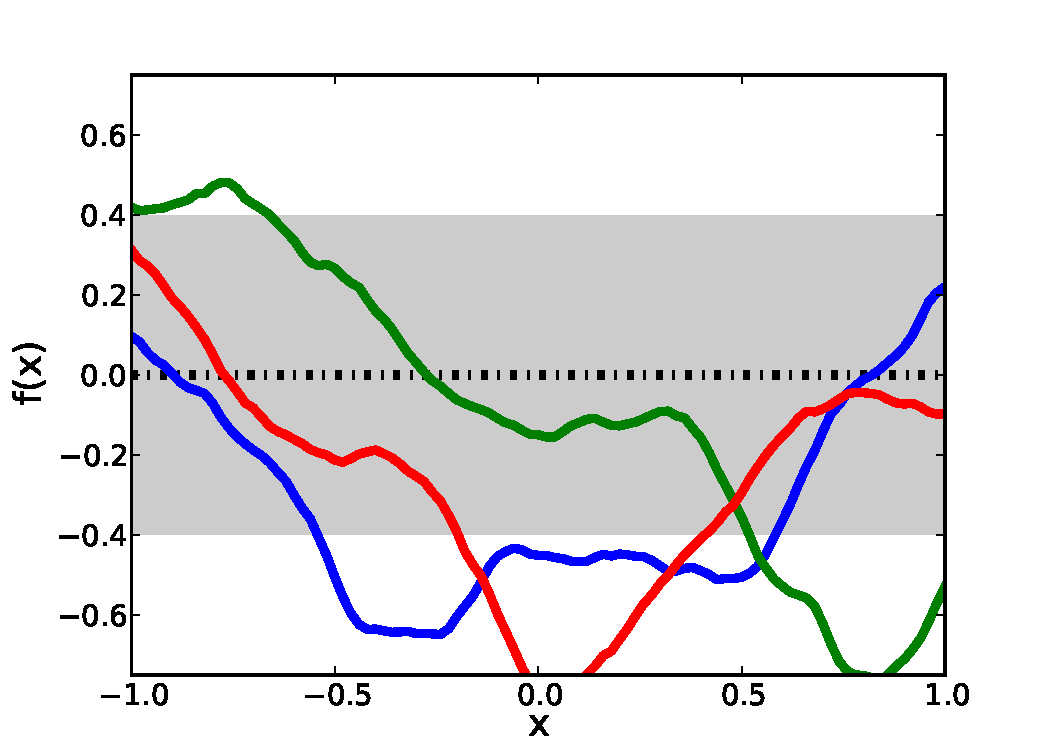
\epsfig{file=figs/nomeshpropose.pdf,width=9cm}
        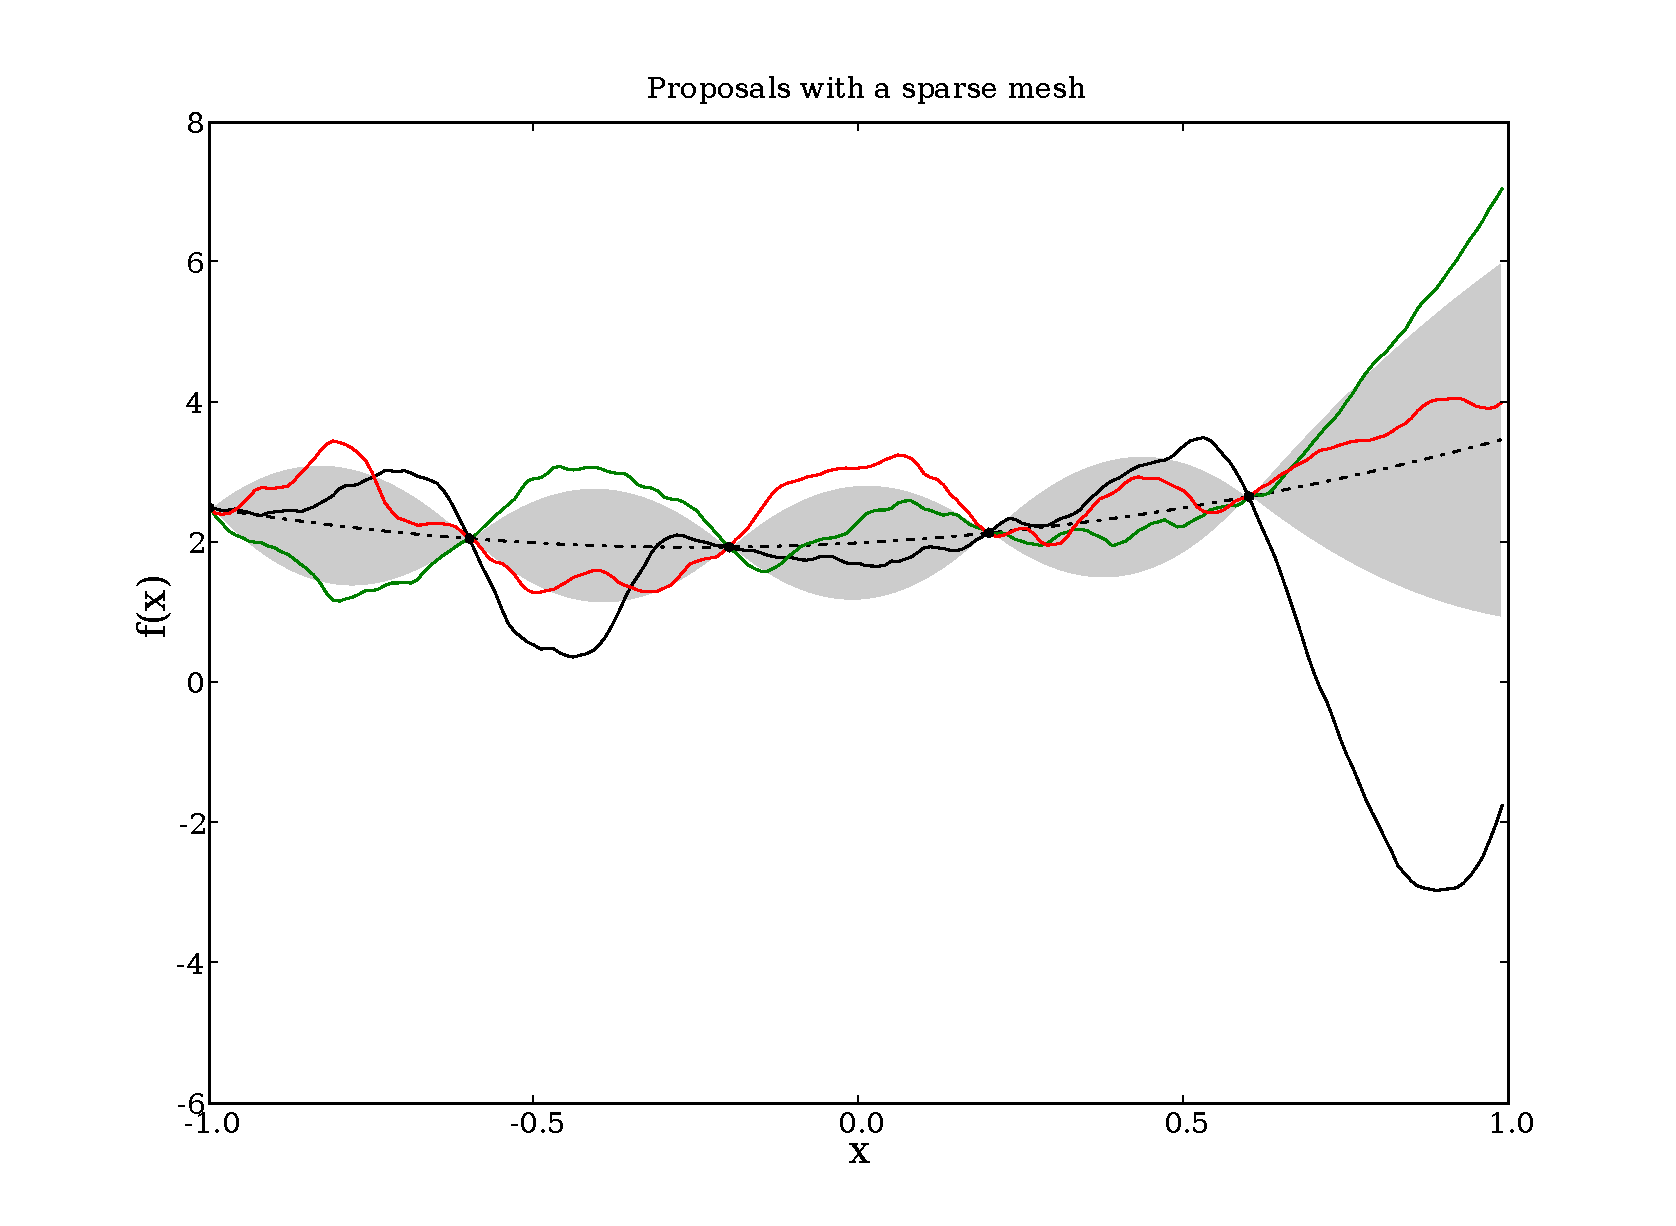
\epsfig{file=figs/lightmeshpropose.pdf,width=9cm}
        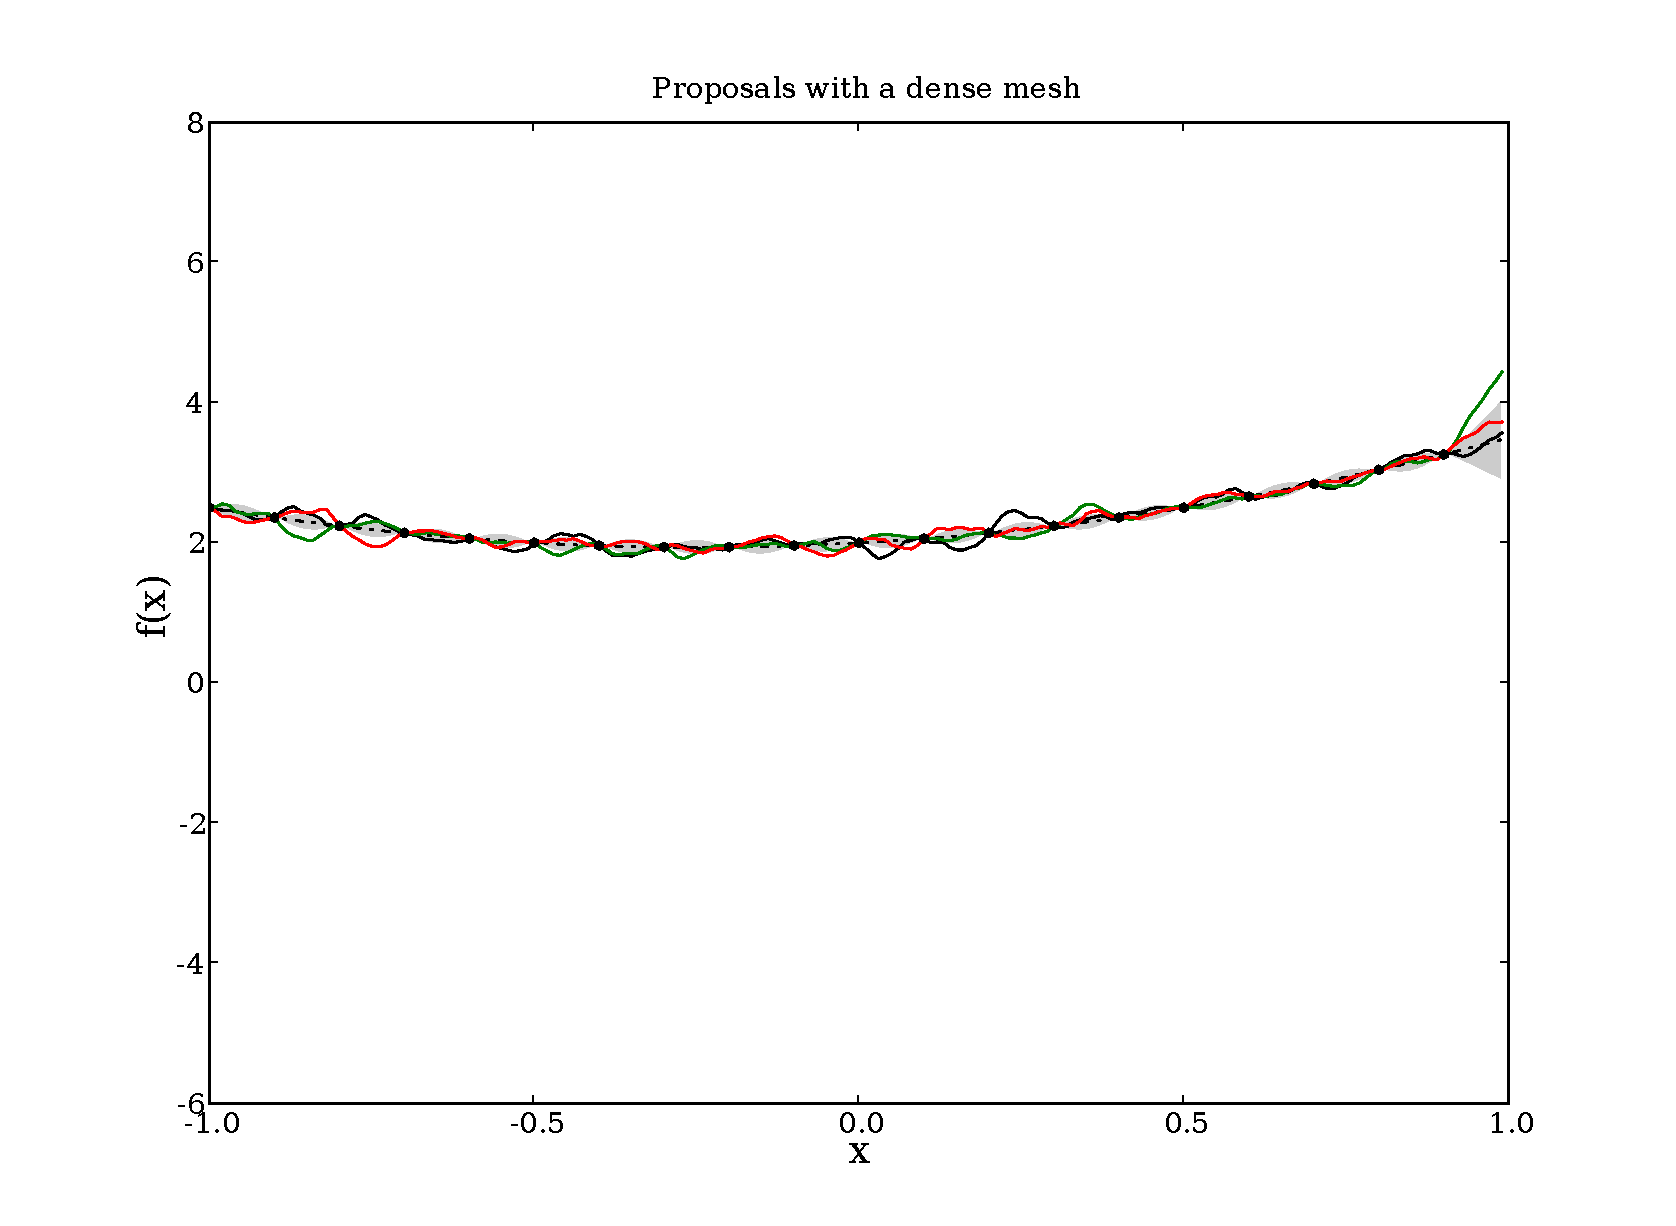
\epsfig{file=figs/densemeshpropose.pdf,width=9cm}
    \caption{Several possible proposals of $\tilde f$ (curves) given proposed values for $f(\texttt{mesh})$ (heavy dots) with no mesh (top), a sparse mesh (middle), and a dense mesh (bottom). Proposal distributions' envelopes are shown as shaded regions, with means shown as broken lines. With no mesh, $\tilde f$ is being proposed from its prior and the acceptance rate will be very low. A denser mesh permits a high degree of control over $\tilde f$, but computing the log-probability will be more expensive.}
    \label{fig:meshpropose}
\end{figure}


\section{The \class{GPNormal} step method}
As we've already seen in other contexts, a \class{GP}'s full conditional distribution is a Gaussian process if its Markov blanket is described by the following probability model:
\begin{eqnarray*}
    K_i |f \sim \textup{N}(f(o_i), V_i) & i=0\ldots n-1\\
    f|M,C\sim\textup{GP}(M,C)
\end{eqnarray*}
In other words, each of its children $K_i$ is normally distributed with variance $V_i$ and mean equal to $f(o_i)$, where $o_i$ is an arbitrary mesh.

In this case, a \texttt{GP} instance $f$ can be handled by the Gibbs step method \class{GPNormal}, which will have much better mixing properties that \class{GPMetropolis}. Its init method takes the following parameters:
\begin{description}
    \item[$f$:] The \texttt{GP} instance to be handled.
    \item[\texttt{obs_mesh:}] An array or array-valued variable giving the observation mesh $o$.
    \item[\texttt{obs_V}:] An array or array-valued variable giving the observation variance $V$.
    \item[\texttt{obs_vals}:] An array or array-valued variable giving the concatenation of the values of the children $K_i$.
\end{description}

\class{GPNormal} doesn't register itself, so it will never be assigned as a default handler. This may change eventually.

\class{GPNormal} doesn't care about $f$'s mesh, because it never has to evaluate $f$'s log-probability. However, a good choice of mesh is important because it will used by the \class{GPParentMetropolis} instances that handle $f$'s mean and covariance parameters.

\section{Example: A simple extension of nonparametric regression}\label{sub:BasicMCMC}
The files \file{examples/PyMCModel.py} and \file{examples/MCMC.py} show \class{GP} and the three step methods listed above in action. The probability model created by \file{examples/PyMCModel.py} is illustrated as a directed acyclic graph in figure \ref{fig:unobservedModel}. If you comment the last line, $f$ will be handled by a default \class{GPMetropolis} instance. If you leave it uncommented, $f$ will be handled by the \class{GPNormal} instance \texttt{S}.

The main script \file{examples/MCMC.py} is mostly devoted to plotting, and its output is shown in figure \ref{fig:MCMCOutput} for both the \class{GPMetropolis} and \class{GPNormal} step methods. Both files are a bit long, so I won't quote them here.
% \verbatiminput{../../examples/gp/PyMCModel.py}

\begin{figure}
    \centering
        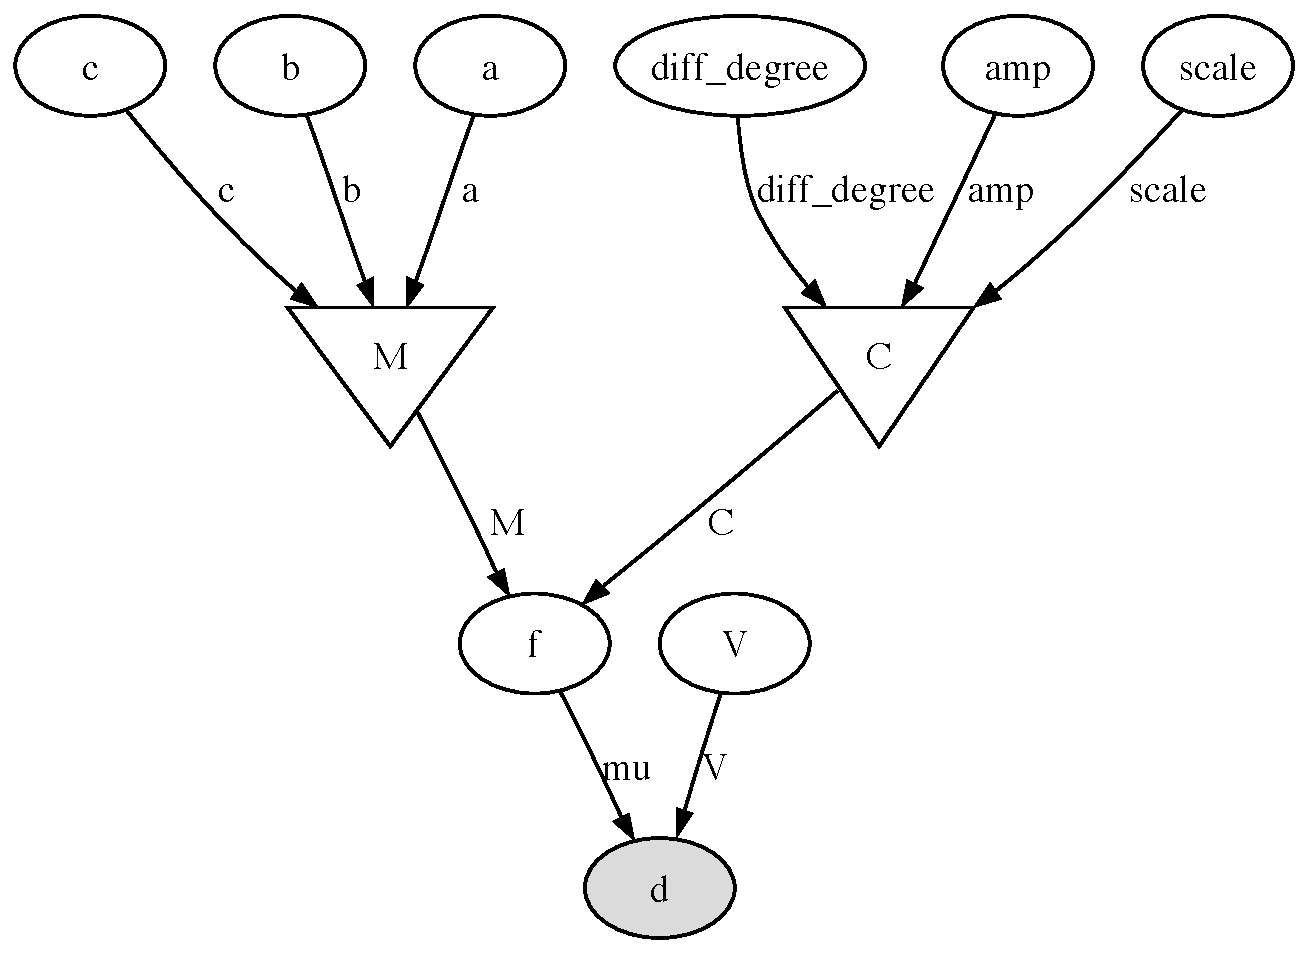
\epsfig{file=figs/unobservedModel.pdf, width=10cm}
    \caption{The PyMC-generated directed acyclic graph representation of the extended nonparametric regression model created by \textsf{`examples/PyMCModel.py'} . Ellipses represent \class{Stochastic} objects (variables whose values are unknown even if their parents' values are known), triangles represent \class{Deterministic} objects (variables whose values can be determined if their parents' values are known), and rectangles represent \class{Stochastic} objects with the \member{isdata} flag set to \member{True} (data). Arrows point from parent to child, and arrow labels show the name assigned to the parent by the child. For instance, \class{C} considers \class{C_amp} to be its `\class{amp}' parameter.}
    \label{fig:unobservedModel}
\end{figure}

\begin{figure}
    \centering
        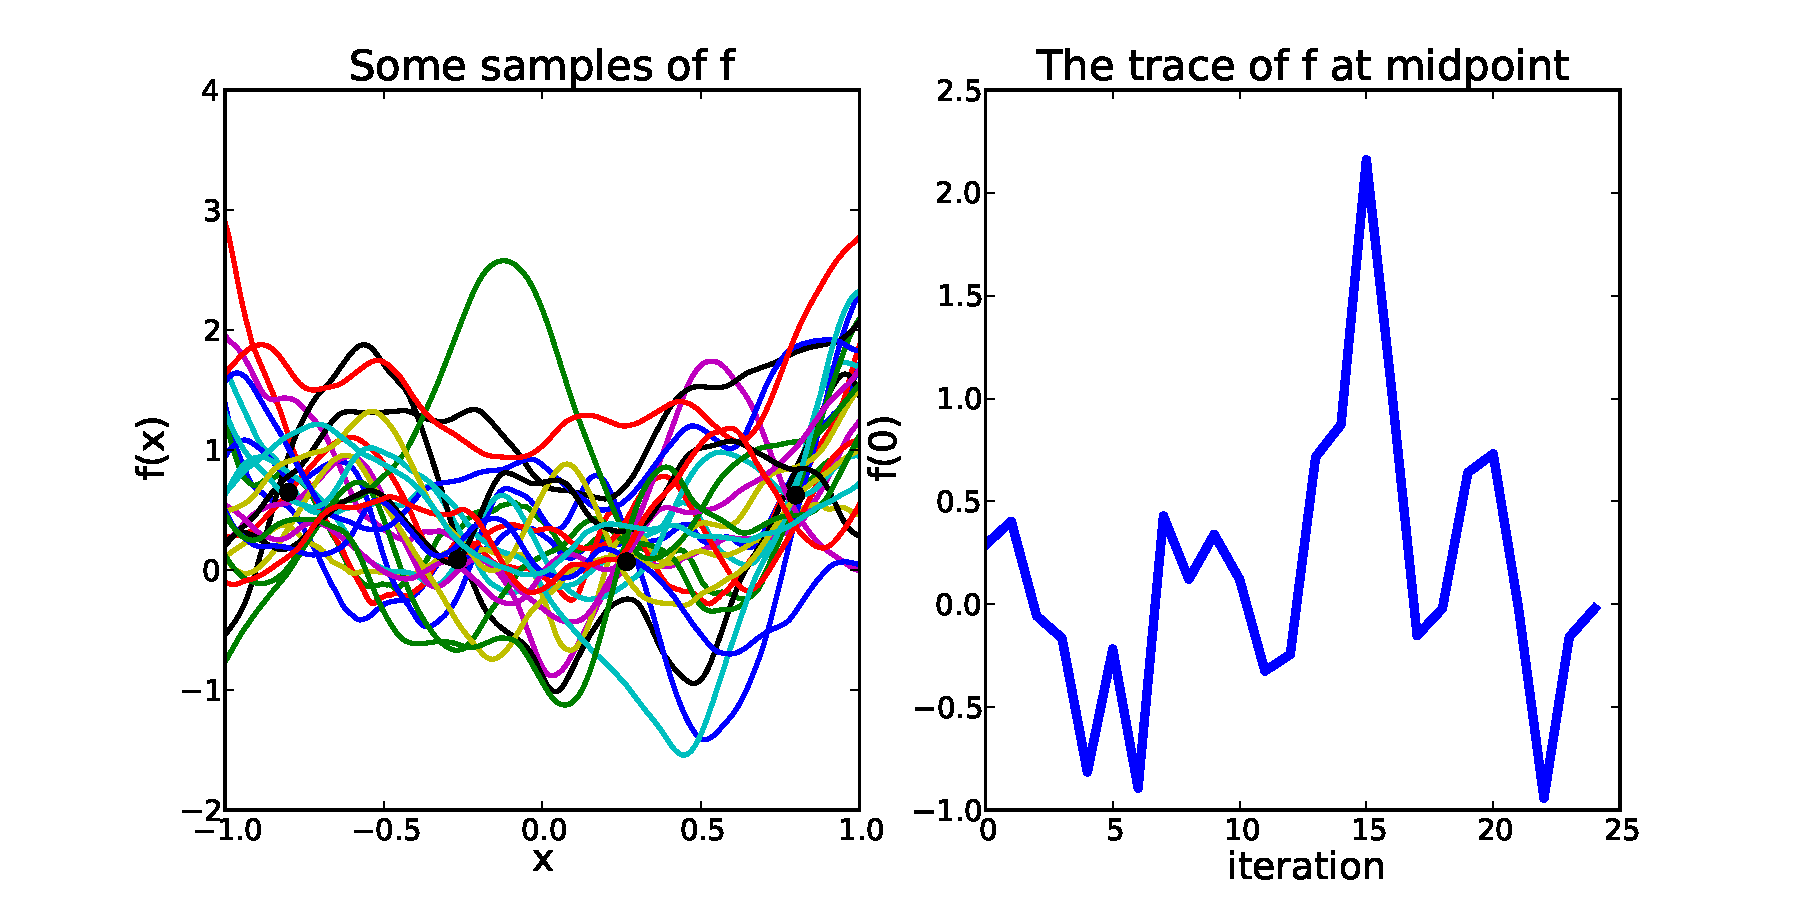
\epsfig{file=figs/gibbsSamples.pdf,width=10cm}
        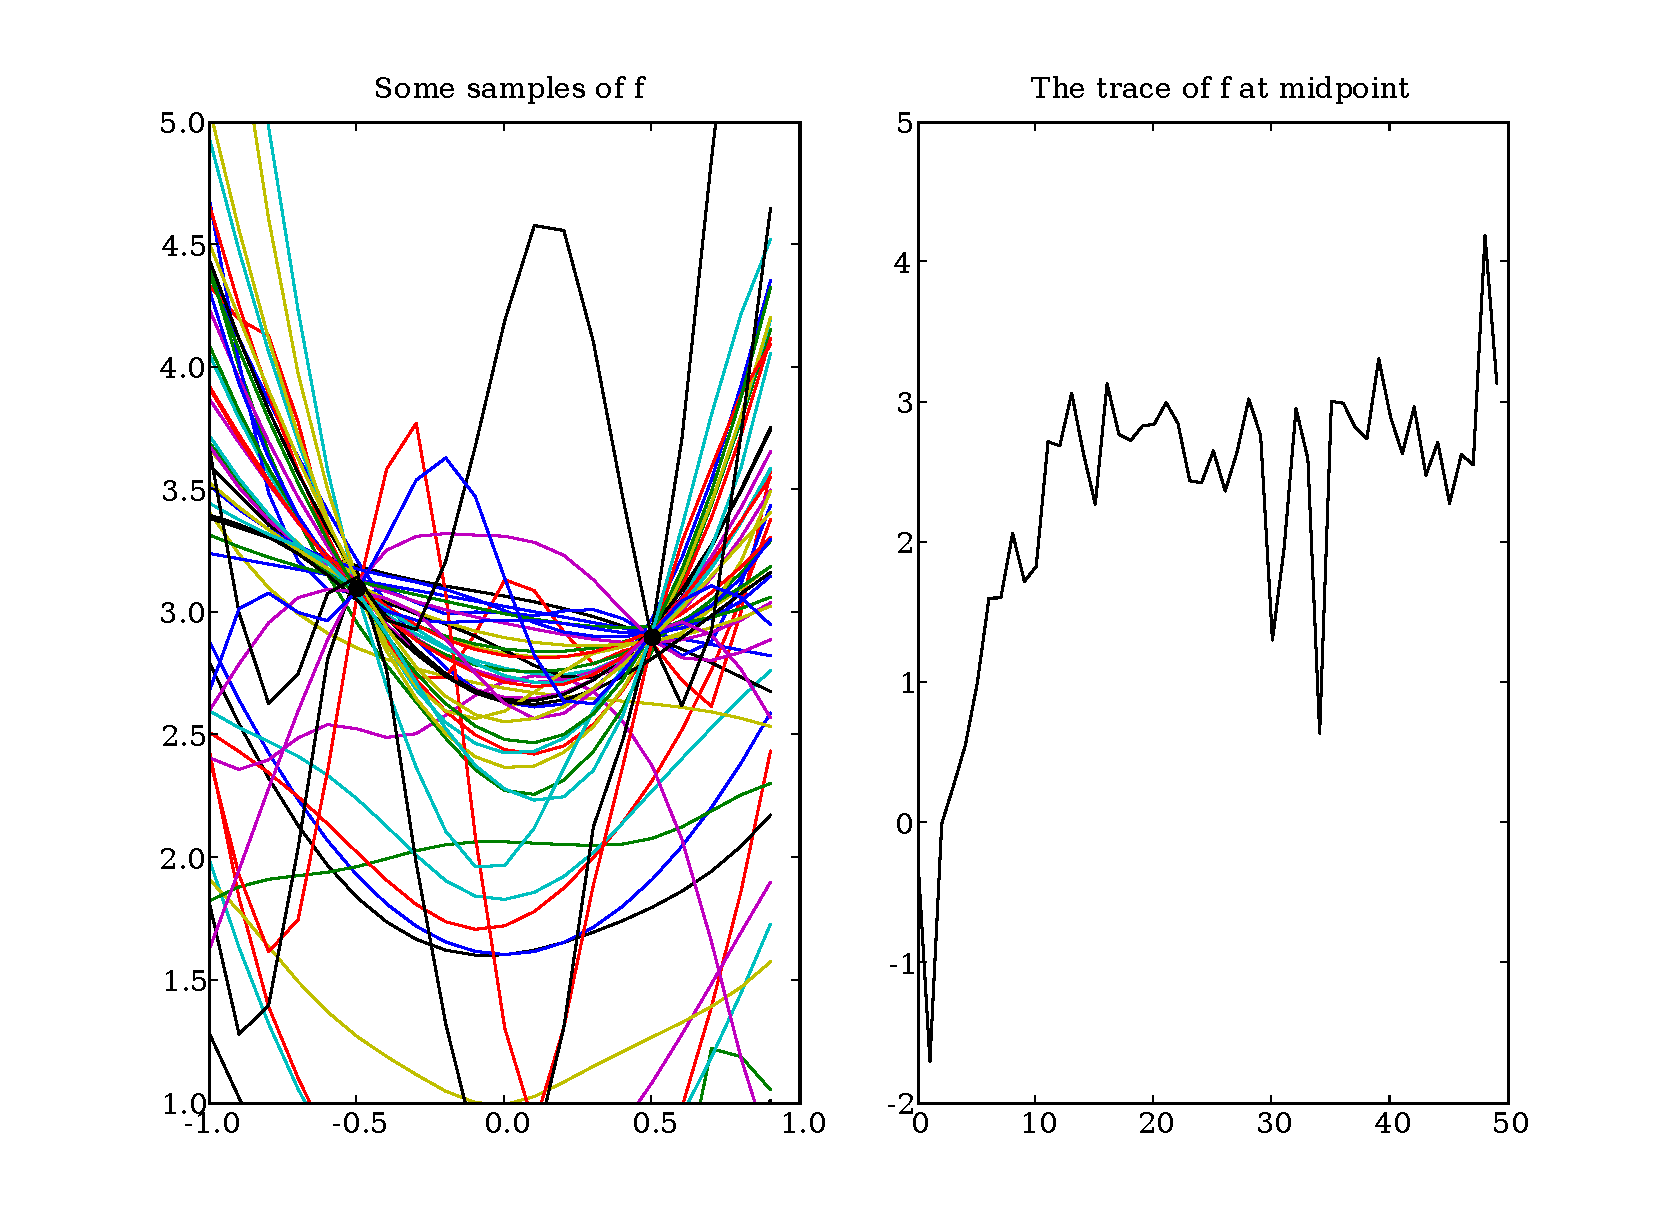
\epsfig{file=figs/metroSamples.pdf,width=10cm}
    \caption{The output of {\sffamily `examples/MCMC.py'} using the \class{GPNormal} (top) and \class{GPMetropolis} (bottom) step methods. Note that the Metropolis samples take several iterations to `burn in' to their dense support, whereas the Gibbs samples jump there more or less immediately. Both the Metropolis and Gibbs samples' jumping distribution is modulated by the value of the prior parameters, which are updated by \class{GPParentMetropolis} step methods.}
    \label{fig:MCMCOutput}
\end{figure}

\section{Example: Munch, Kottas and Mangel's stock-recruitment study}\label{sub:MMKMCMC}

\begin{figure}
    \centering
        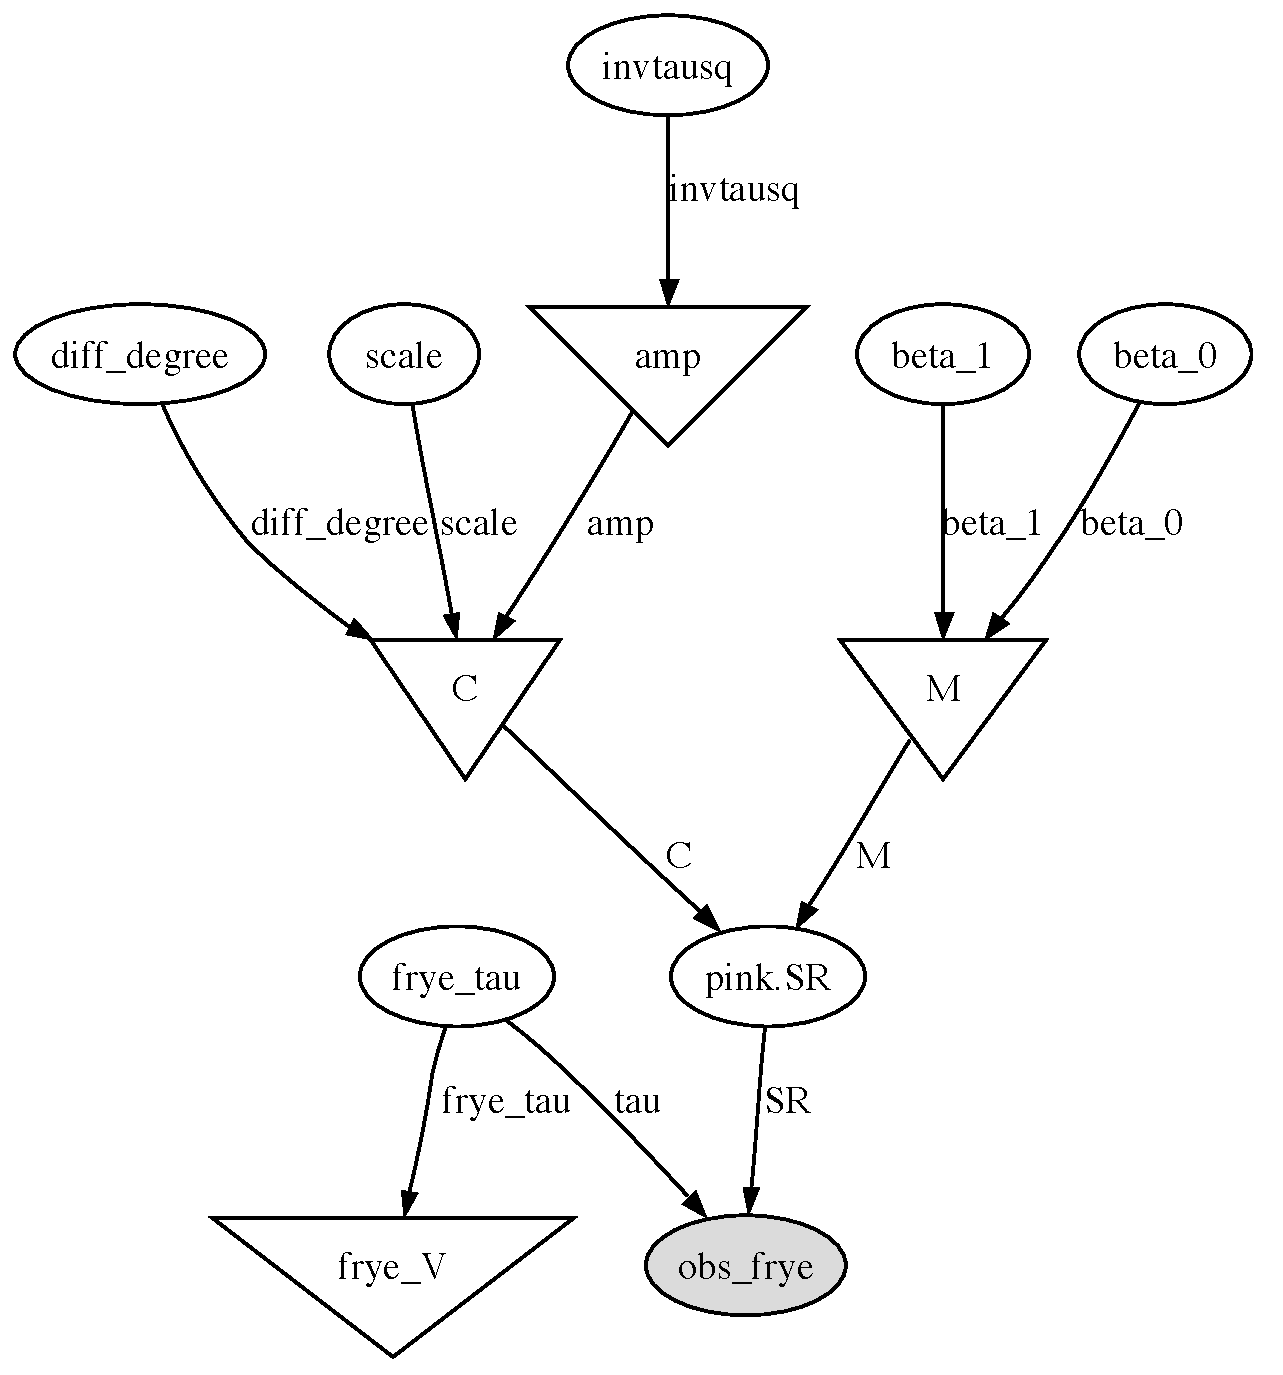
\epsfig{file=figs/MKMsalmon.pdf, width=10cm}
    \caption{A PyMC-generated directed acyclic graph representation of the probability model in (\ref{eqn:MMKModel}), which is implemented in file \textsf{`examples/more_examples/MKMSalmon/salmon_sampler.py'}. A very similar probability model was used by Munch, Kottas and Mangel to infer stock-recruitment functions for three salmonid species. The label `\texttt{pink.SR}' indicates that this particular model corresponds to the pink salmon (\emph{Onchorhynchus gorbuscha}) data. Note that two coordinate transformations are implemented using PyMC deterministic variables. This technique can help lazy programmers avoid transforming priors by hand, and in less trivial cases it can save computation by caching the transformed parameters.}
    \label{fig:MMKsalmonmodel}
\end{figure}

\begin{figure}
    \centering
        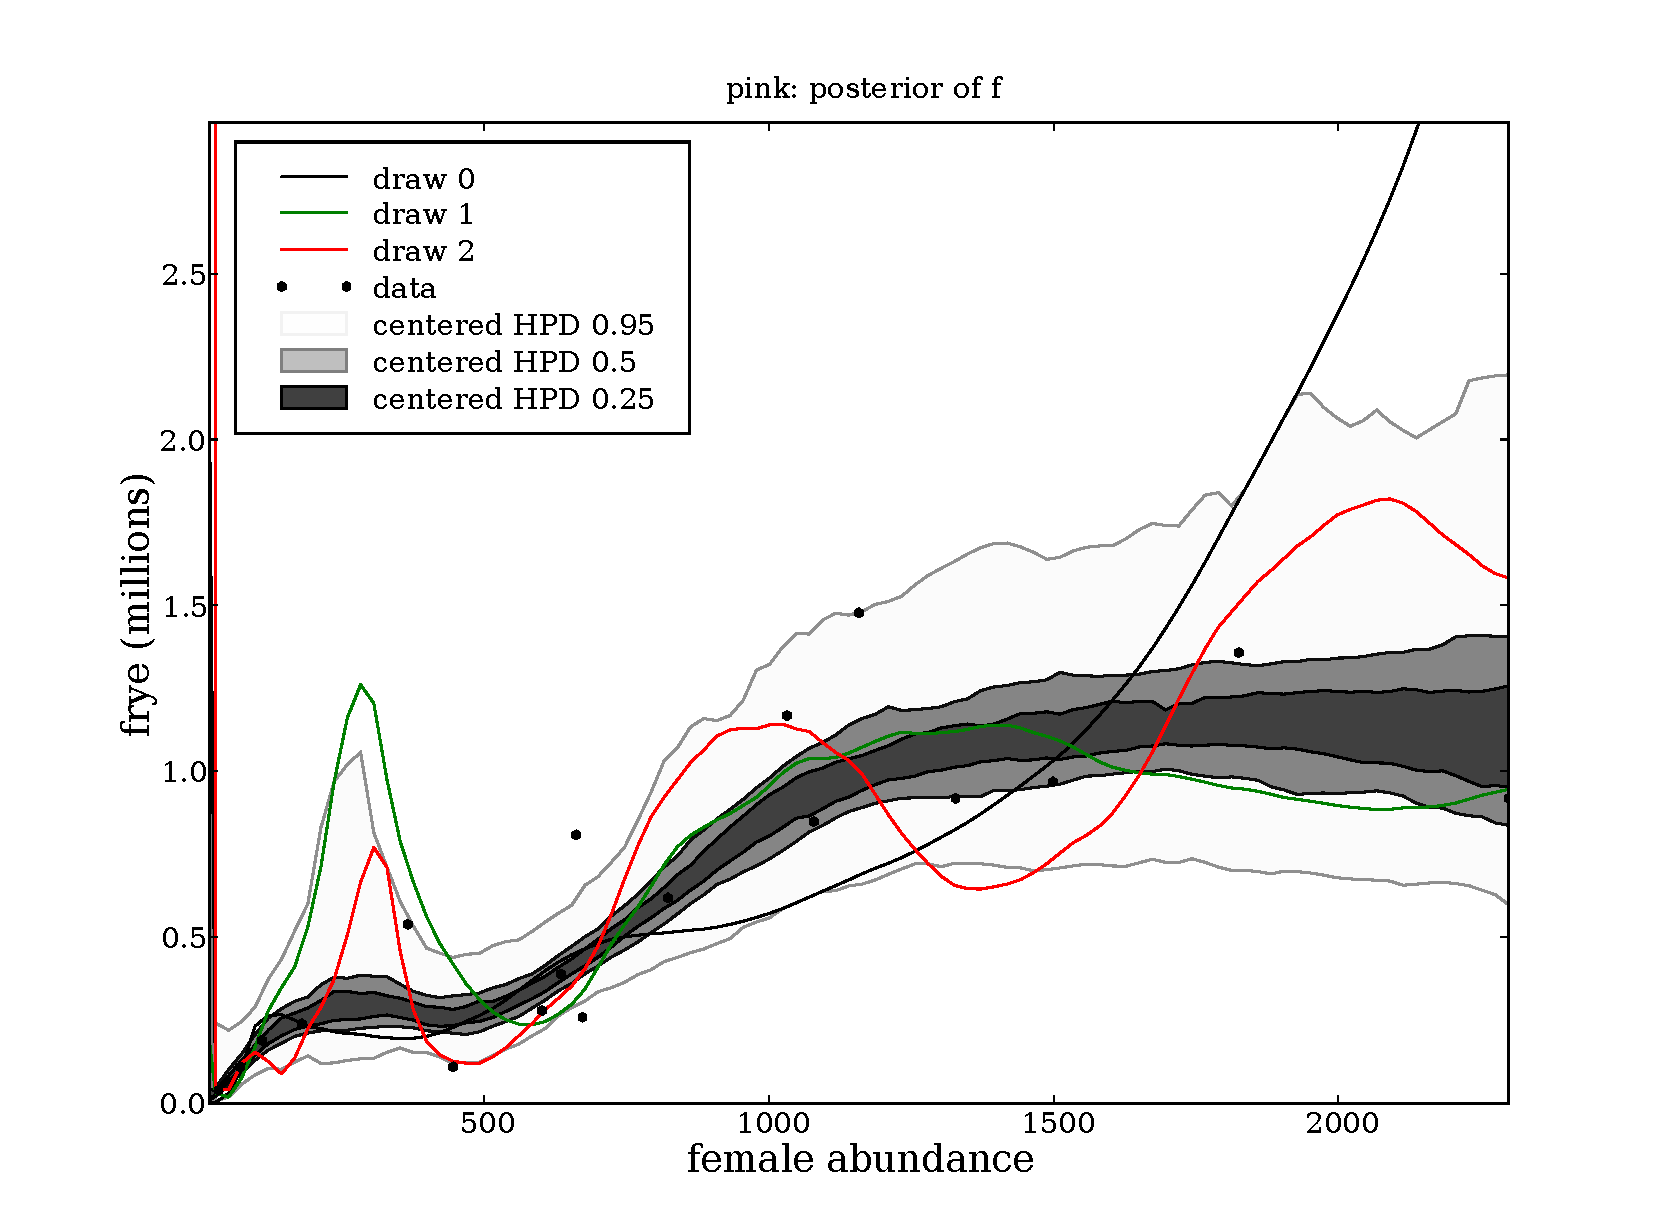
\epsfig{file=figs/pinkfpost.pdf, width=10cm}
    \caption{The posterior of the stock-recruitment function for pink salmon (\emph{Onchorhynchus gorbuscha}). The data are shown as heavy black dots. The centered 95\%, 50\% and 25\% posterior probability intervals are shown as shaded regions. Three draws from the posterior are plotted.}
    \label{fig:pinkfpost}
\end{figure}

\begin{figure}
    \centering
        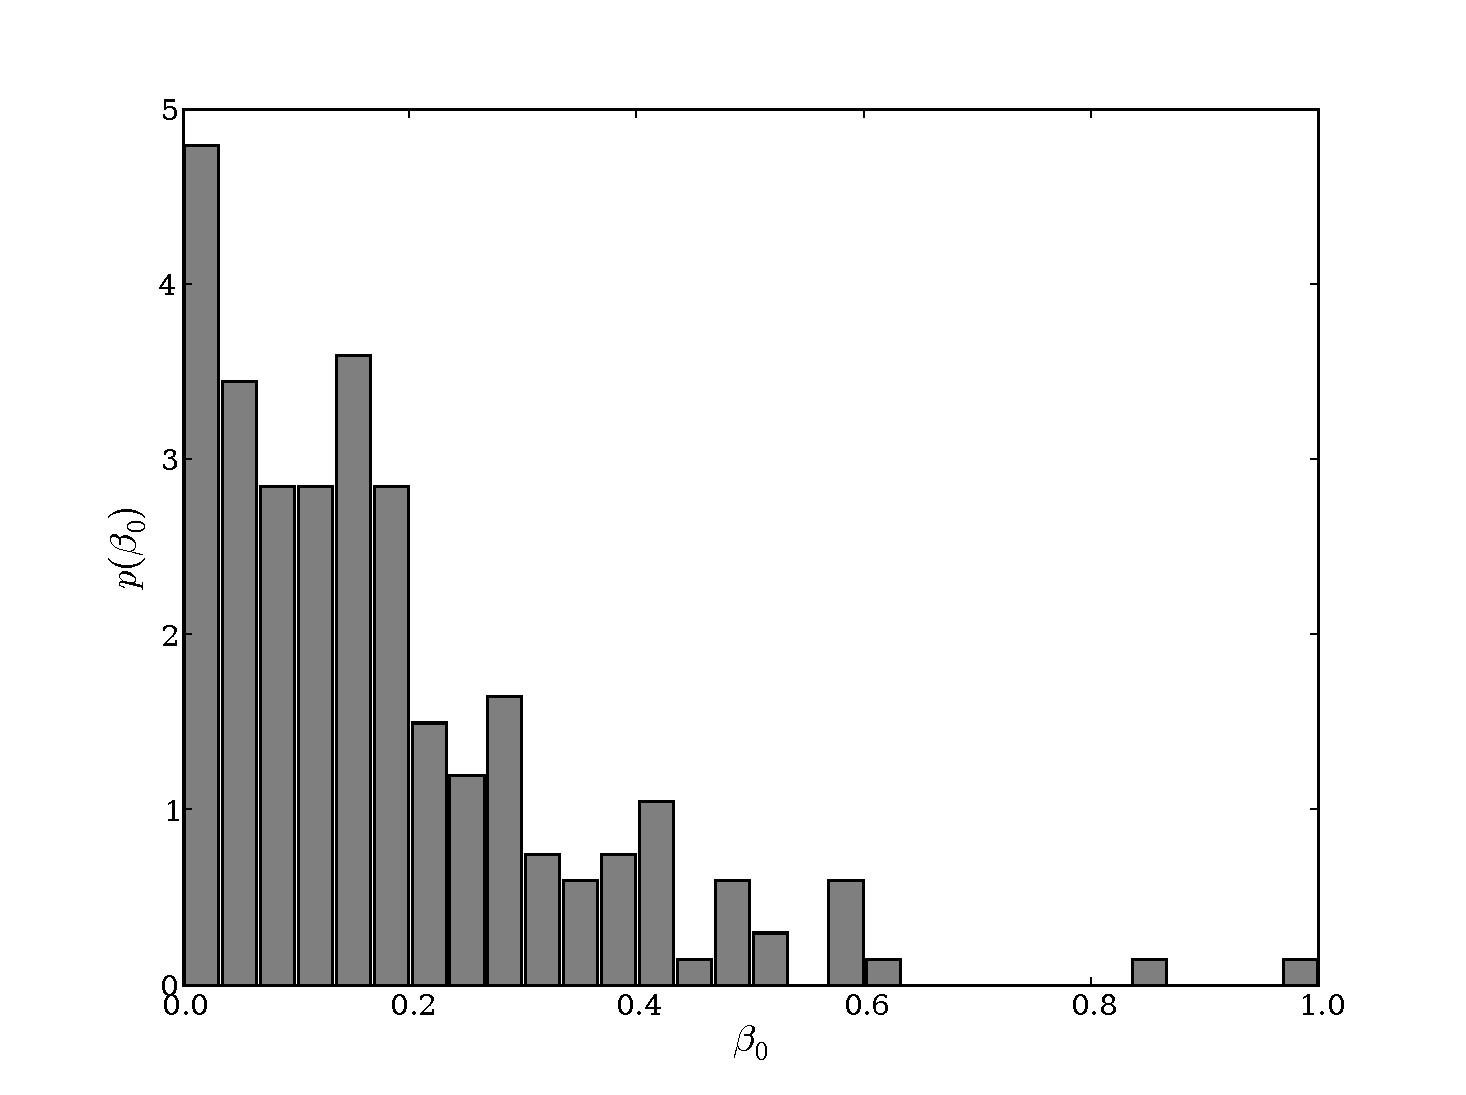
\epsfig{file=figs/pinkbeta0post.pdf, width=5cm}
        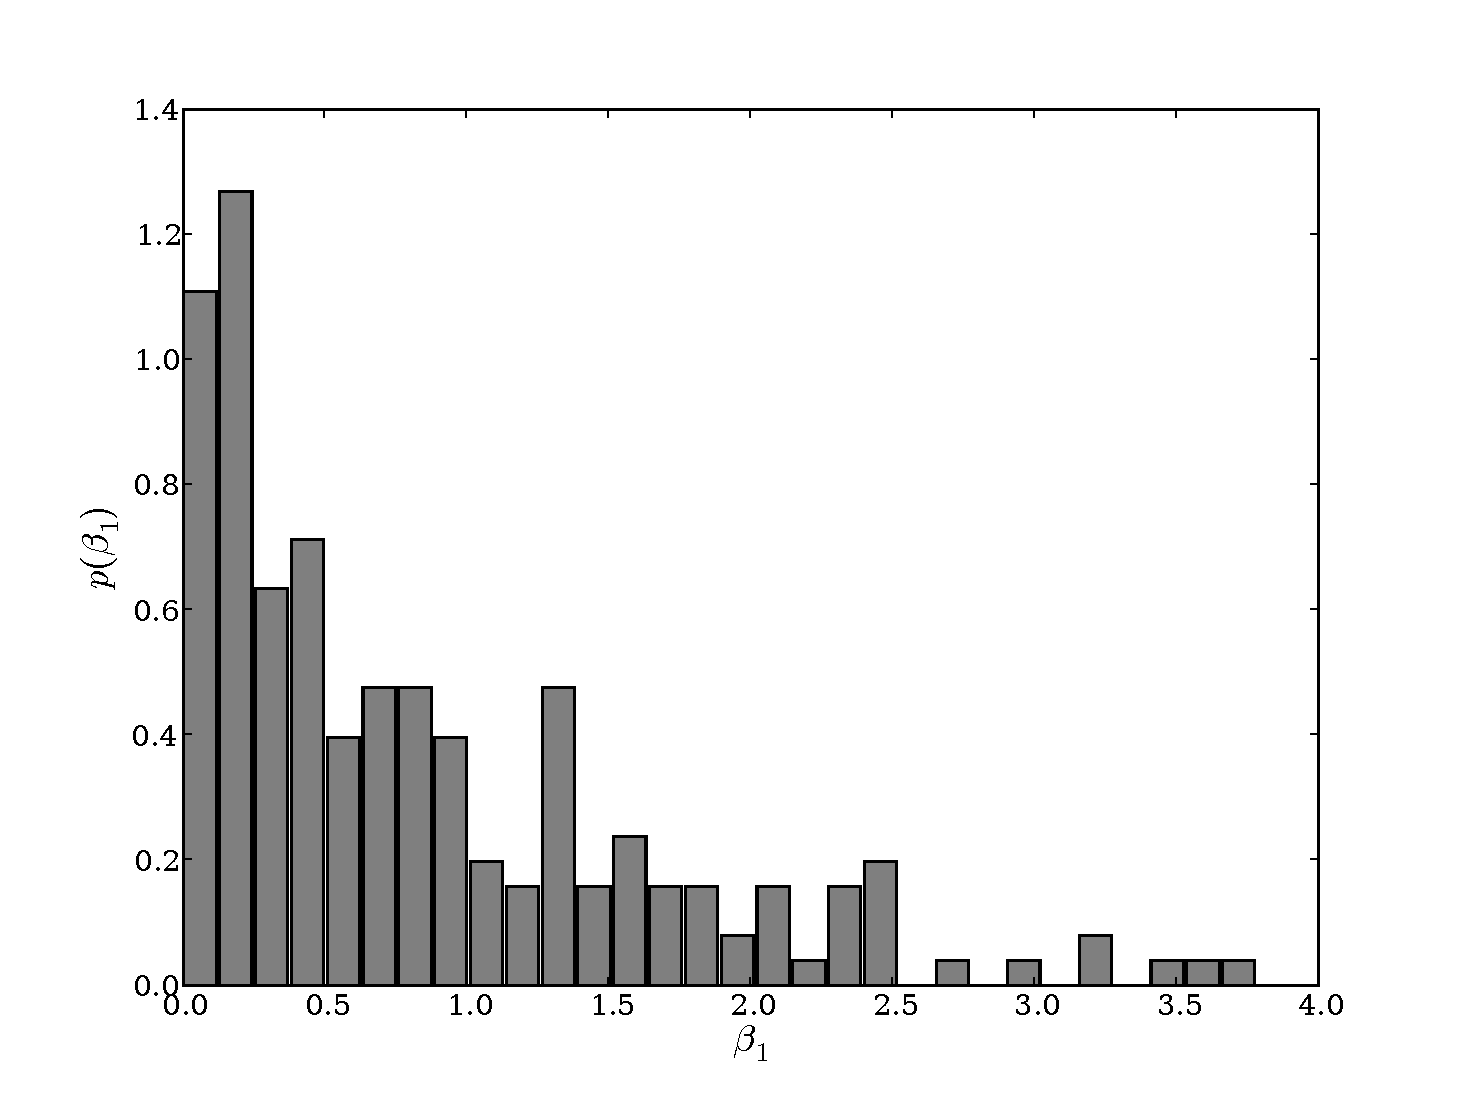
\epsfig{file=figs/pinkbeta1post.pdf, width=5cm}
        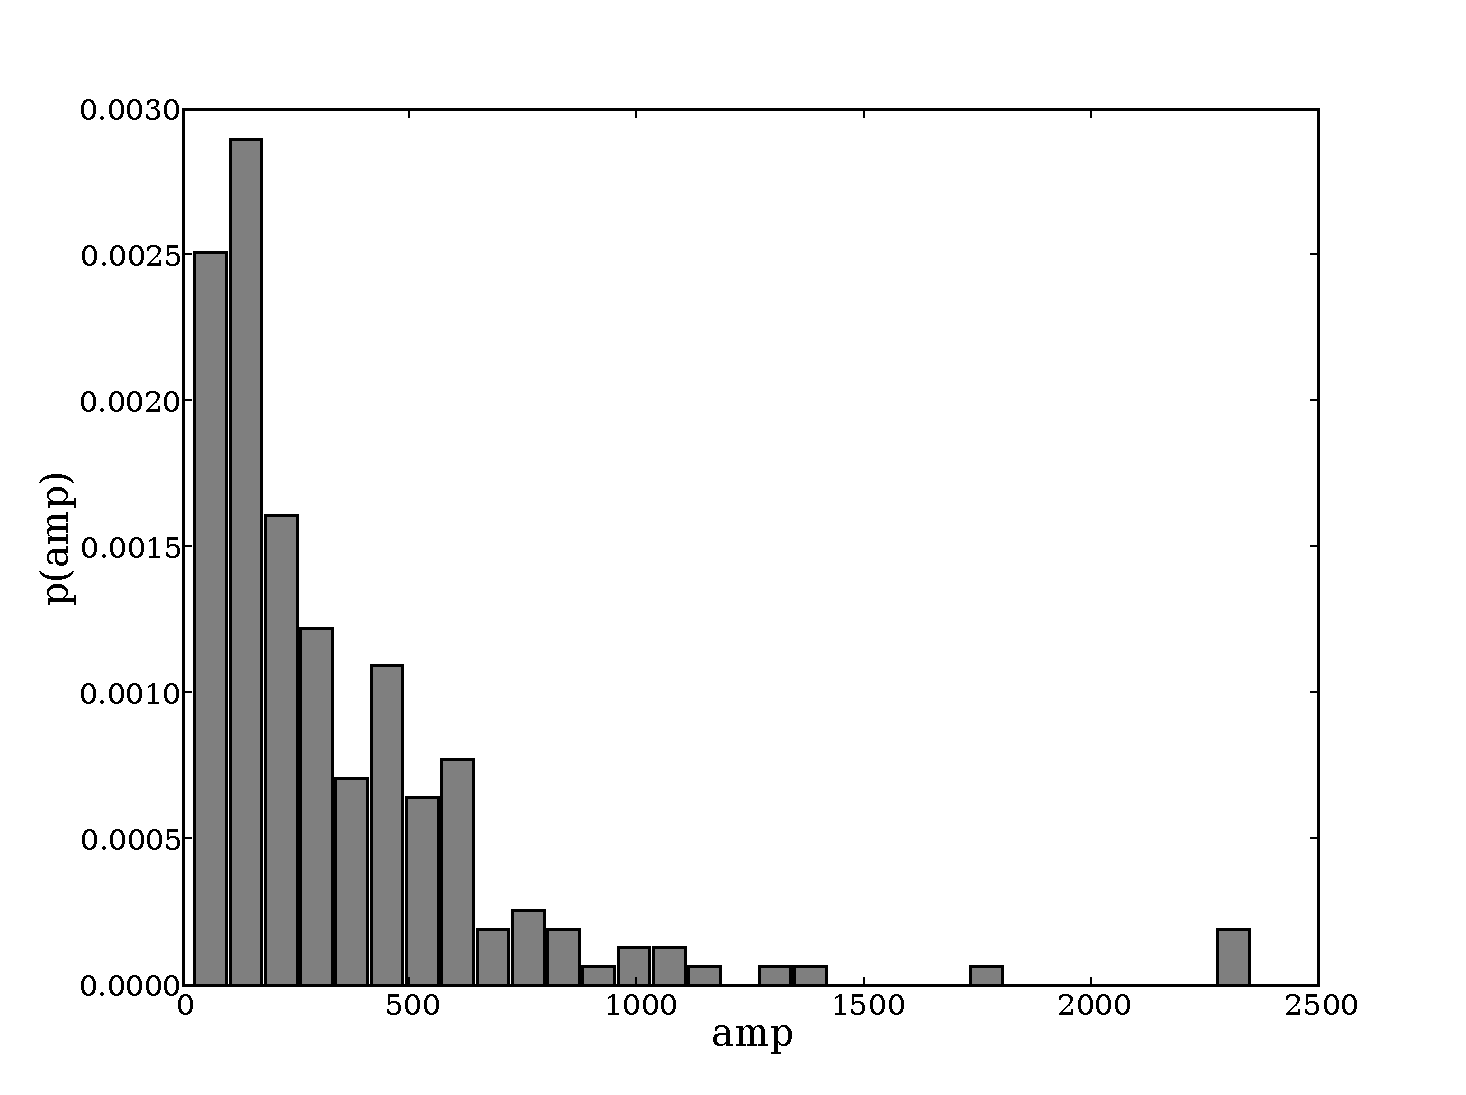
\epsfig{file=figs/pinkamppost.pdf, width=5cm}
        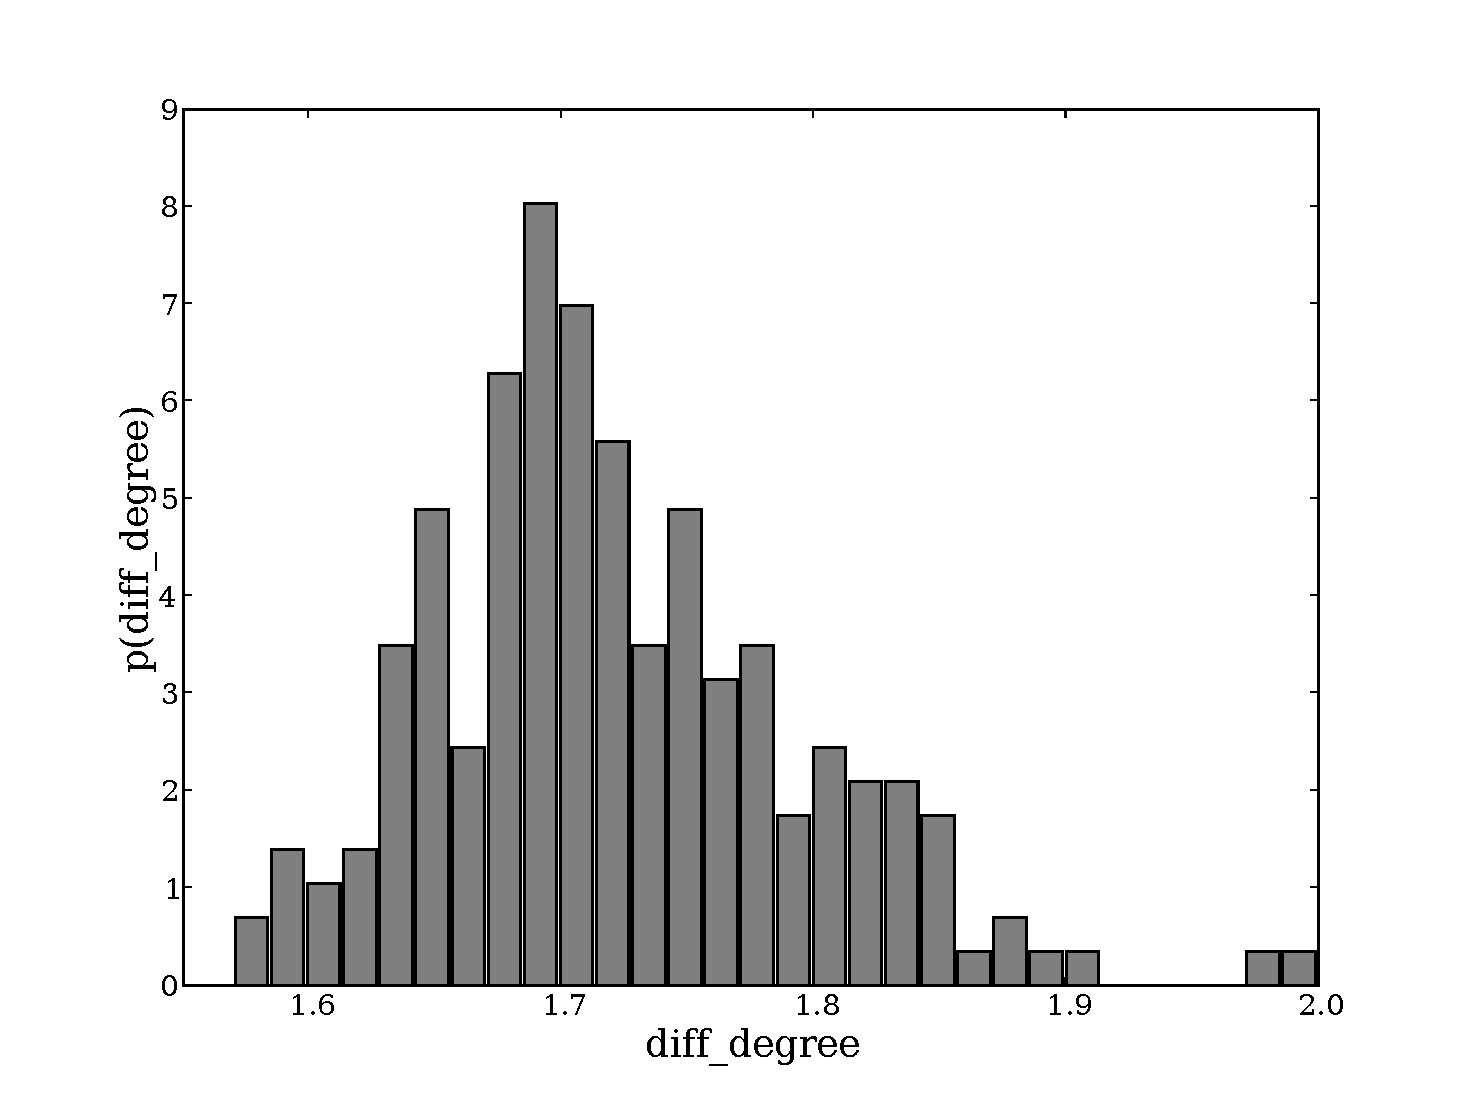
\epsfig{file=figs/pinkdiffdegreepost.pdf, width=5cm}
        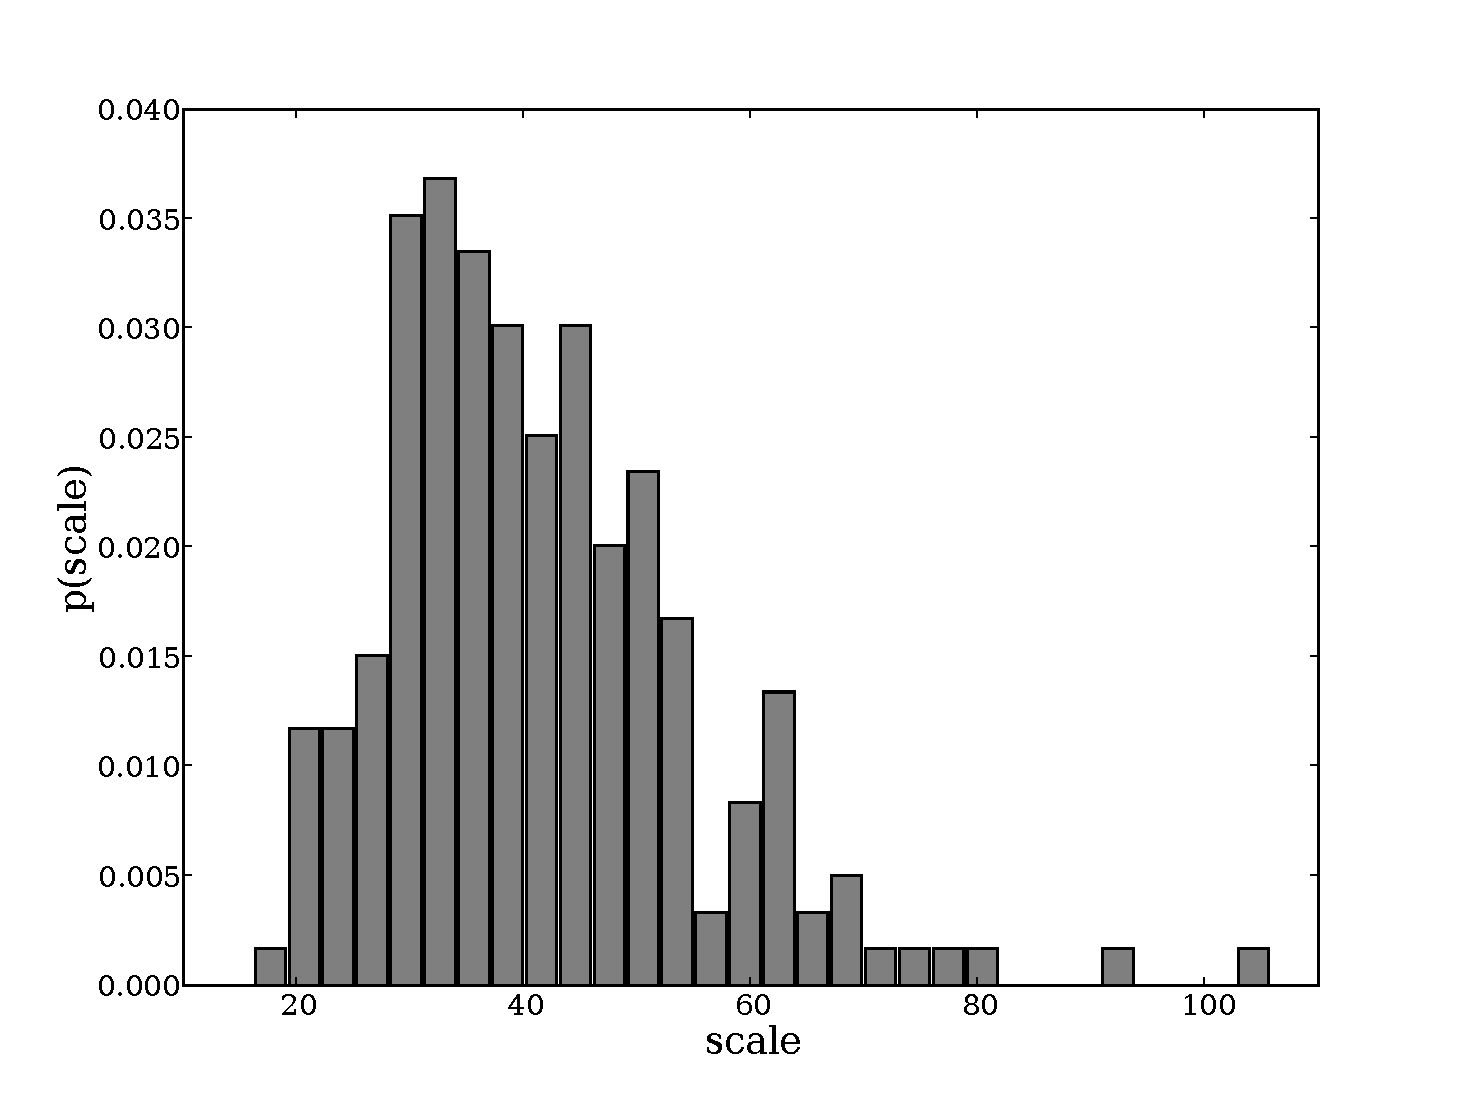
\epsfig{file=figs/pinkscalepost.pdf, width=5cm}
        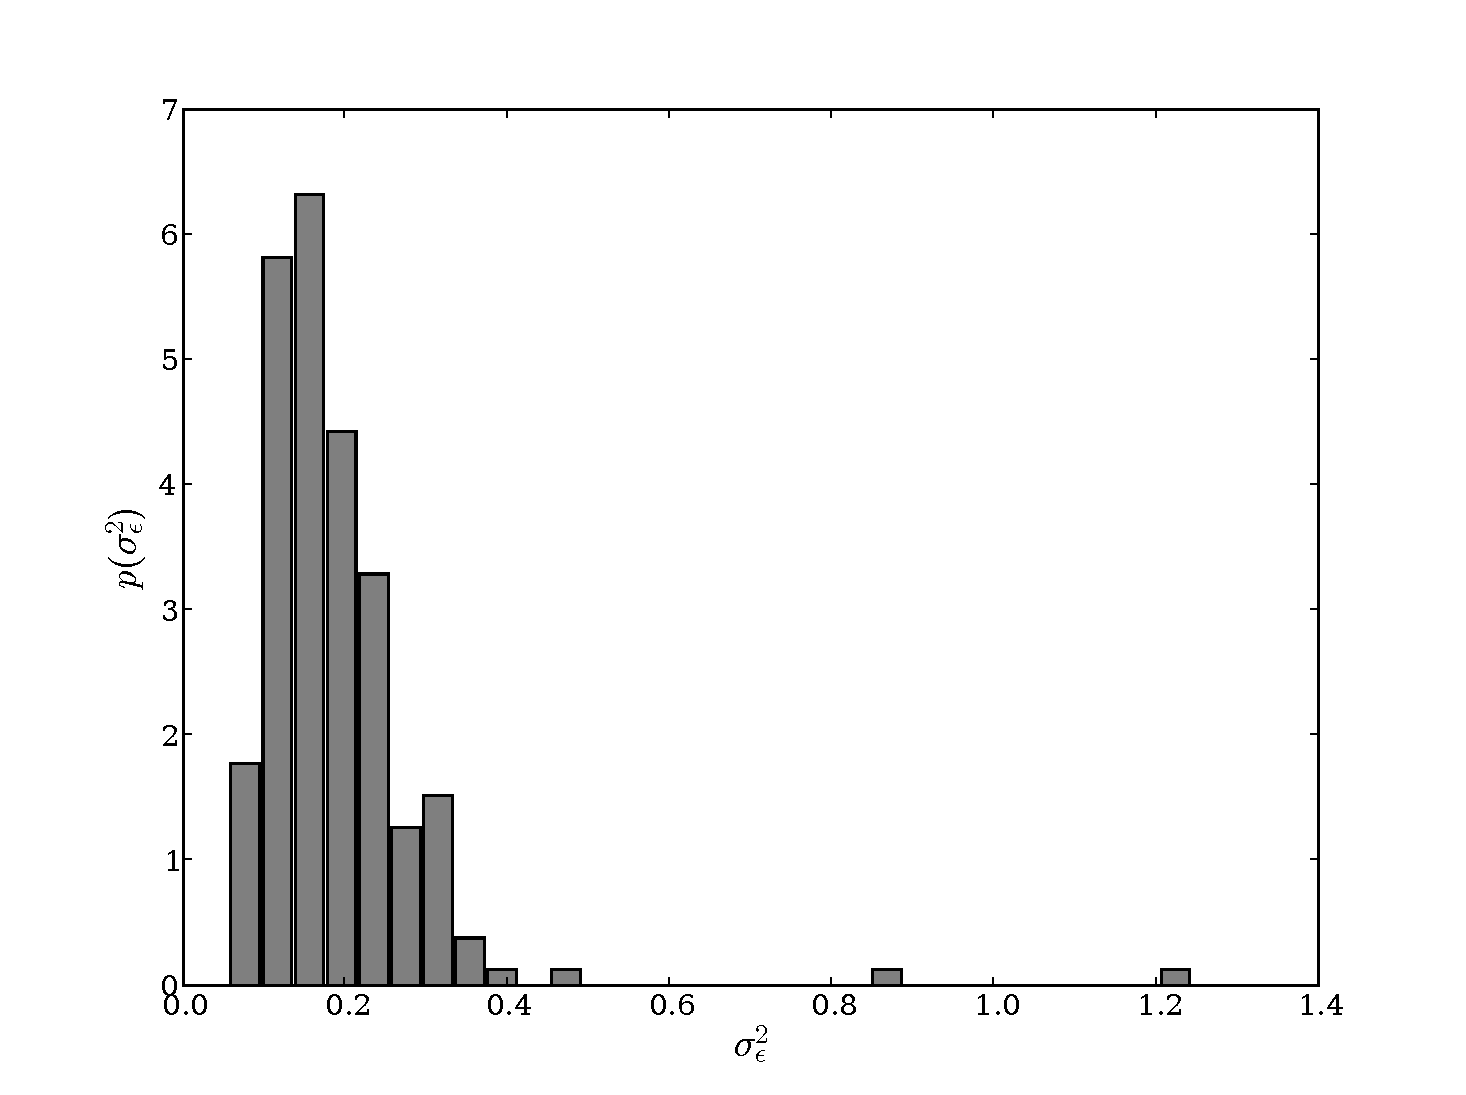
\epsfig{file=figs/pinkVpost.pdf, width=5cm}
    \caption{The marginal posterior distributions of the mean and covariance parameters of the stock-recruitment function for pink salmon (\emph{Onchorhynchus gorbuscha}).}
    \label{fig:pinkparams}
\end{figure}

We now have the tools to duplicate Munch, Kottas and Mangel's \cite{mmk} stock-recruitment results. The full probability we'll use follows. It is like Munch, Kottas and Mangel's probability model, but we will use a Mat\`ern covariance function. Here \texttt{SR} is the stock-recruitment function, C is its covariance and M is its mean.
\begin{equation}
    \label{eqn:MMKModel}
    \begin{array}{ll}
        \texttt{frye}[i] \stackrel{\tiny{\textup{ind}}}{\sim} \textup{N}(exp(\mathtt{SR}(\log(\mathtt{abundance}[i]))), V),& i=1\ldots n\\
        \texttt{SR}\sim \textup{GP}(M,C)& \\
        M:x\rightarrow \beta_0+\beta_1 \log(x)&\\
        C:x,y\rightarrow \texttt{matern.euclidean}(x,y;\ \texttt{diff_degree},\texttt{amp},\texttt{scale})&\\
        V,\ \beta_0,\ \beta_1,\ \texttt{diff_degree},\ \texttt{amp},\ \texttt{scale} \sim \texttt{priors}.&
    \end{array}
\end{equation}
The `priors' can be found by reading their paper (except the prior on \texttt{diff_degree}, which I chose based on what seems reasonable to me) or by reading the file \file{examples/more_examples/MMKSalmon/salmon_sampler.py}. This file contains a PyMC \class{Sampler} subclass called \class{SalmonSampler}, which reads in the data, creates a probability model incorporating the data, and provides some plotting methods.

Note that this model differs from the model in section \ref{sub:MMKregression} in that we're putting a Gaussian process prior on the stock-recruitment function in log-log space, so conditioning its value at zero isn't an option.

The probability model \class{SalmonSampler} creates is visualized as a directed acyclic graph in figure \ref{fig:MMKsalmonmodel}. Munch, Kottas and Mangel specify priors for $\texttt{amp}^{-2}$ and $V^{-1}$, and I've used PyMC deterministic variables to conveniently implement the transformations rather than changing variables manually. The posterior distribution of \texttt{SR} for the pink salmon (\emph{Onchorhynchus gorbuscha}) is shown in figure \ref{fig:pinkfpost}, and the posterior of the mean and covariance parameters for the same species are shown in figure \ref{fig:pinkparams}.

% \section{Example: Ellner, Seifu and Smith's blowfly study}\label{sub:ESSMCMC}
%
% \textbf{I haven't been able to get this one to mix yet.} The model is:
% \begin{eqnarray*}
%     \textup{data}_t \stackrel{\tiny{\textup{ind}}}{\sim}(A_t, V)\\
%     A_t = B(A_{t-\tau})\psi_{t-\tau} - D(A_{t-1})\phi_{t-1}, & t>\tau\\
%     B \sim \textup{GP}(sx\exp(-rx), C_B) \\
%     D \sim \textup{GP}(mx, C_D) \\
%     \psi_t \stackrel{\tiny{\textup{iid}}}{\sim}\textup{lognorm}(\mu_\phi,V_\phi) \\
%     \phi_t \stackrel{\tiny{\textup{iid}}}{\sim}\textup{lognorm}(\mu_\phi,V_\phi)\\
%     C_B = \textup{Mat\`ern}(\sigma_B,\nu_B,\phi_B) \\
%     C_D = \textup{Mat\`ern}(\sigma_D,\nu_D,\phi_D)   \\
%     A_{1\ldots\tau},r,s,m,\textup{covariance parameters},\mu_\phi,\mu_\psi,V_\phi,V_\psi,V \sim \textup{priors},
% \end{eqnarray*}
% and I assumed $\tau$ fixed for purposes of the demo. The DAG schematic is shown in figure \ref{fig:ESSblowflymodel}.
%
% What happens is the following: when $B$ and $D$ have mean zero, the model burns in and mixes badly. When they have the mean functions parametrized above, the amplitude of their covariance params get very small; the model is preferring the simpler parametric version, since it can explain the data as well as the nonparametric version. This would make a great demo for both the importance of a flexible mean function and the natural parsimony of Bayesian statistics, but I can't even get the parametric version mixing and don't have time for week-long runs. We'll see what happens with this.
%
% \begin{figure}
%     \centering
%         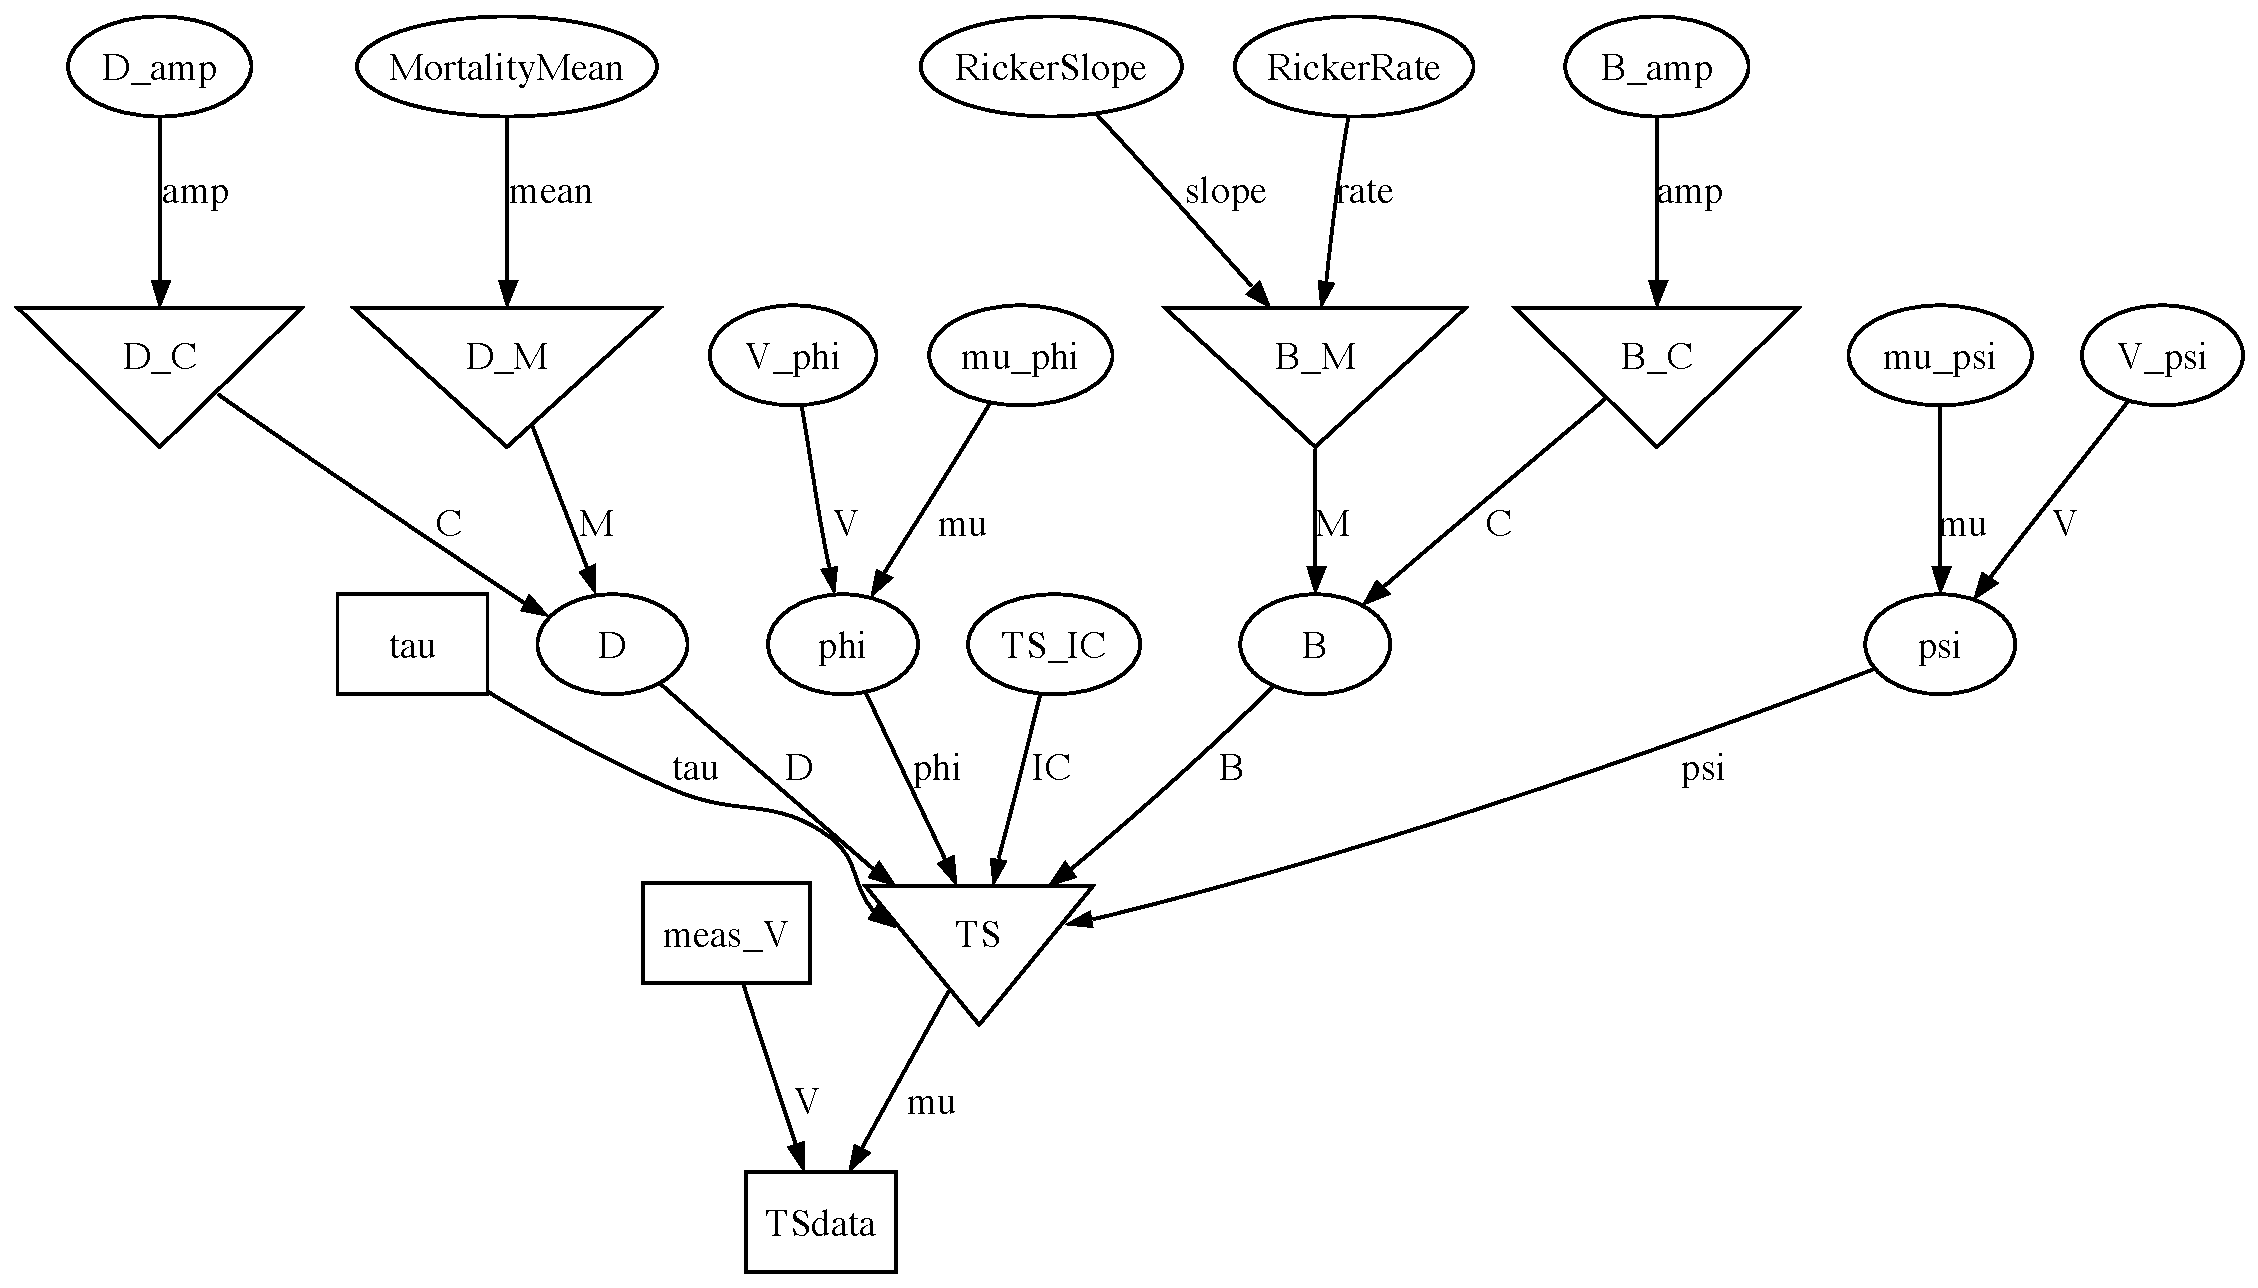
\epsfig{file=figs/ESSblowfly.pdf,width=15cm}
%     \caption{The model for Ellner, Seifu and Smith's \cite{ess} blowfly data.}
%     \label{fig:ESSblowflymodel}
% \end{figure}
%
% % \begin{figure}
% %     \centering
% %         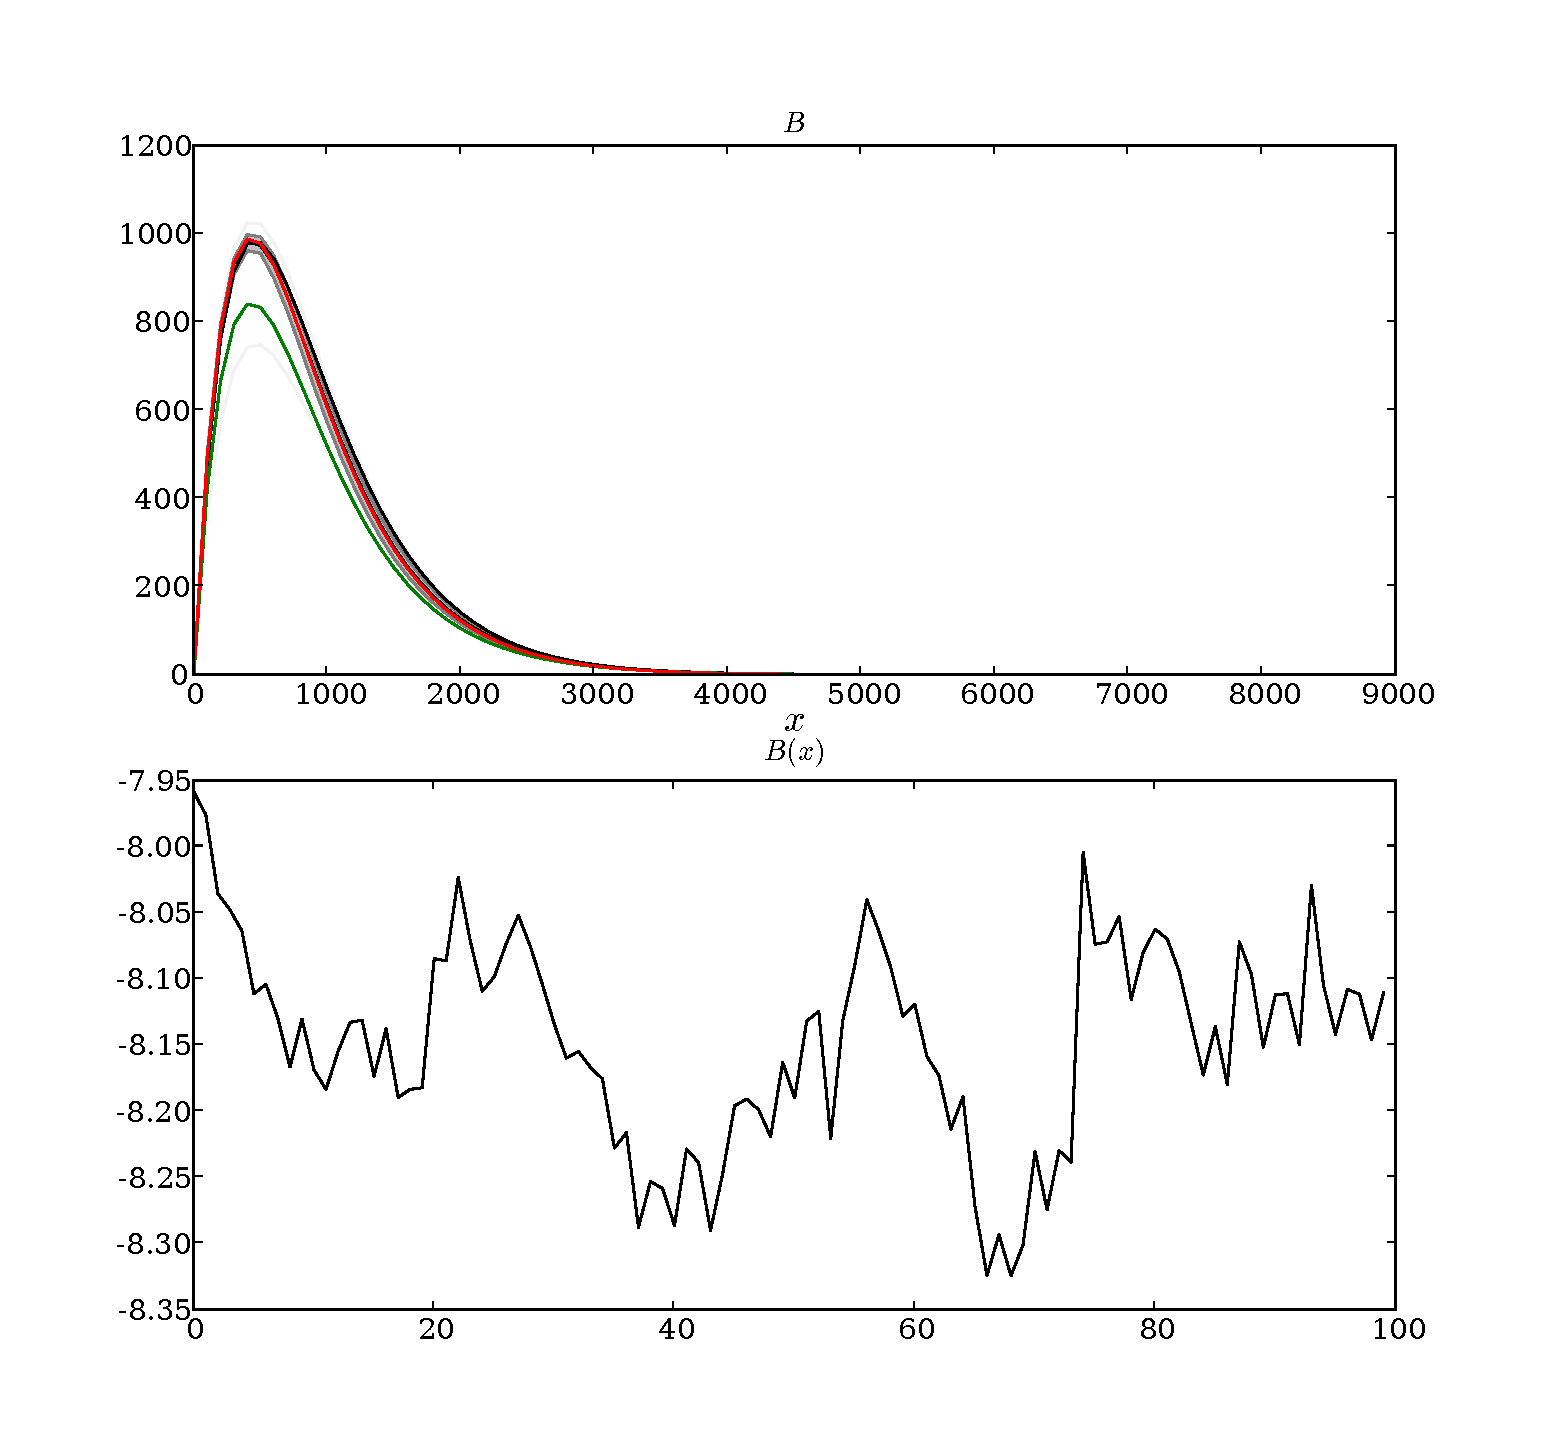
\epsfig{file=figs/ESSBPosterior.pdf,width=10cm}
% %         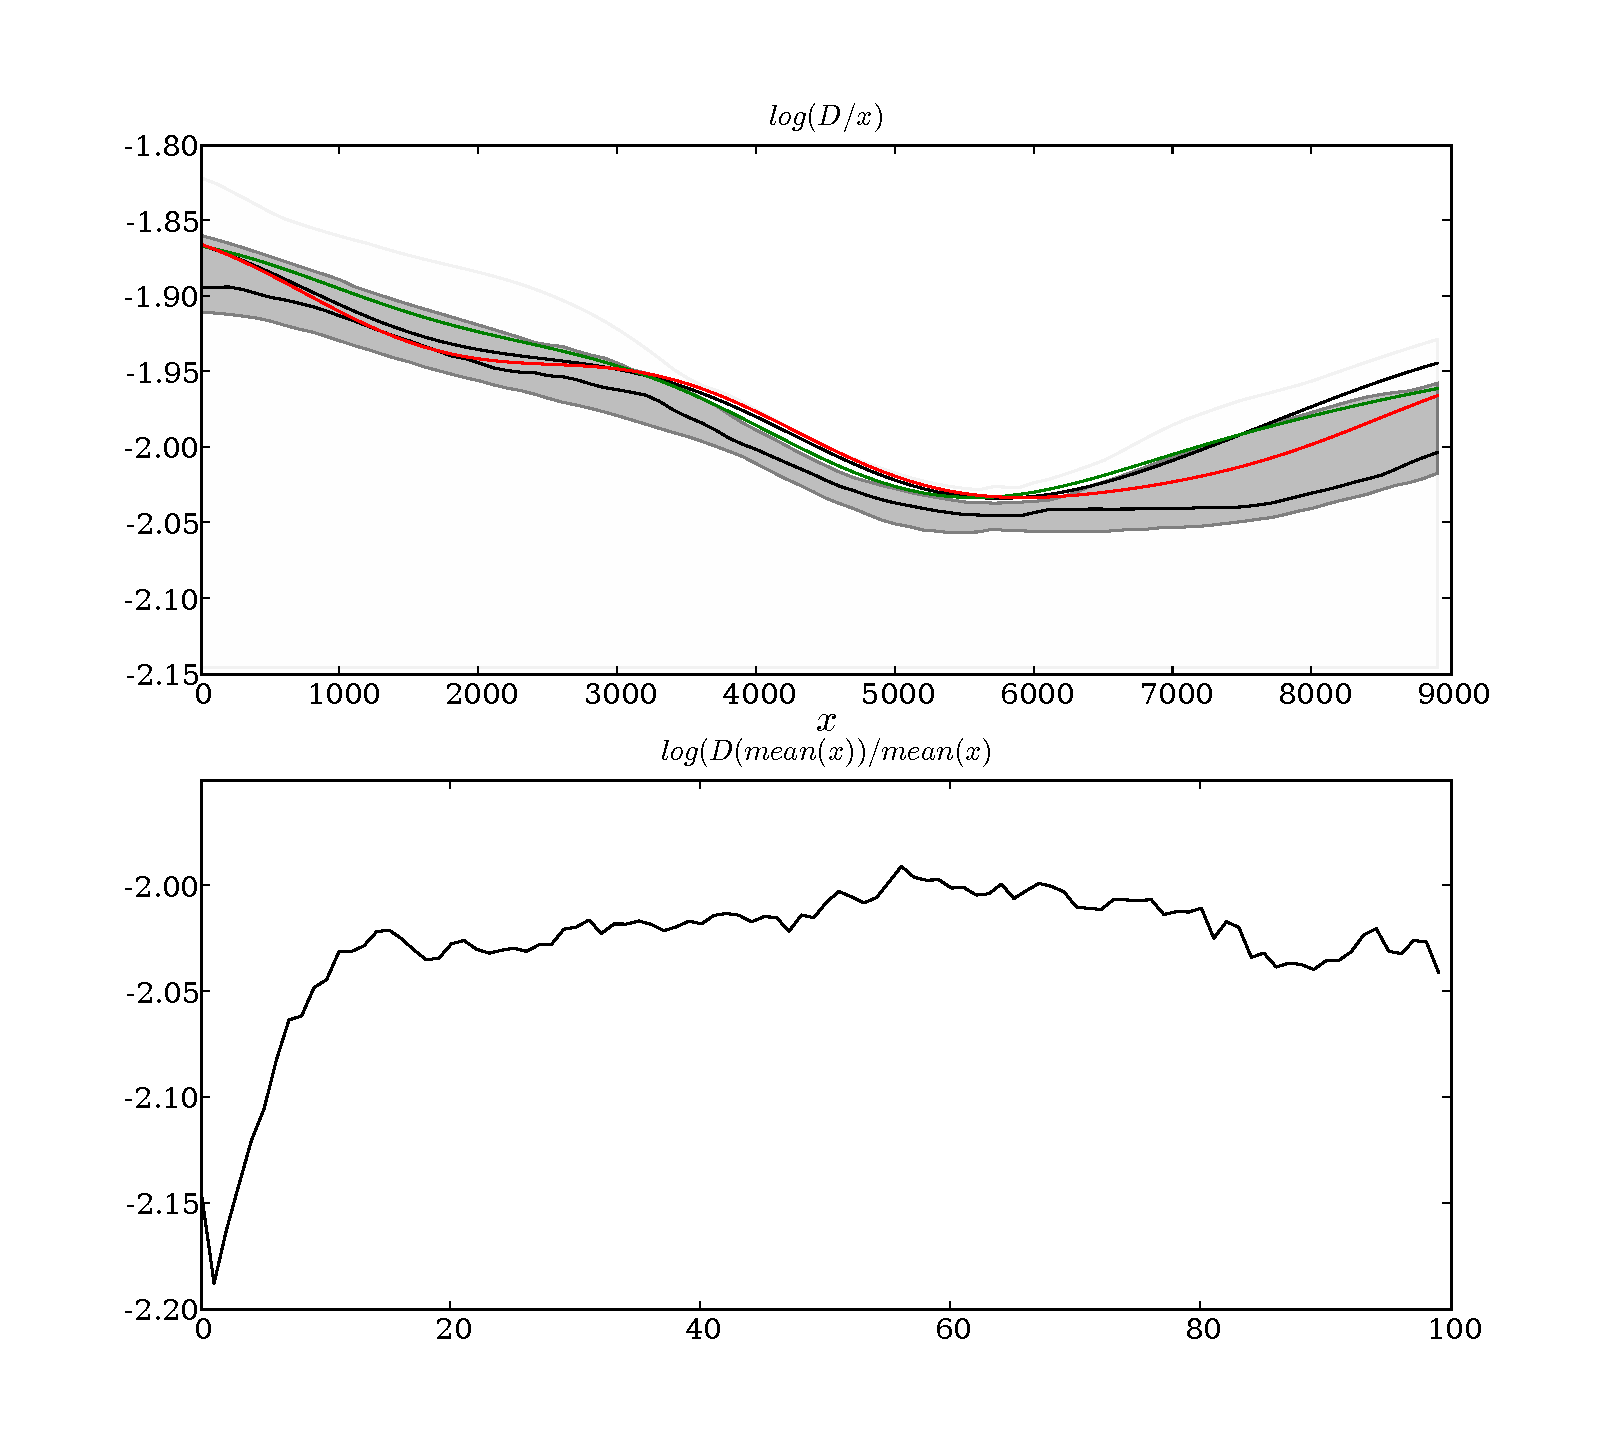
\epsfig{file=figs/ESSDPosterior.pdf,width=10cm}
% %     \caption{caption}
% %     \label{fig:ESSBD}
% % \end{figure}
% %
% % \begin{figure}
% %     \centering
% %         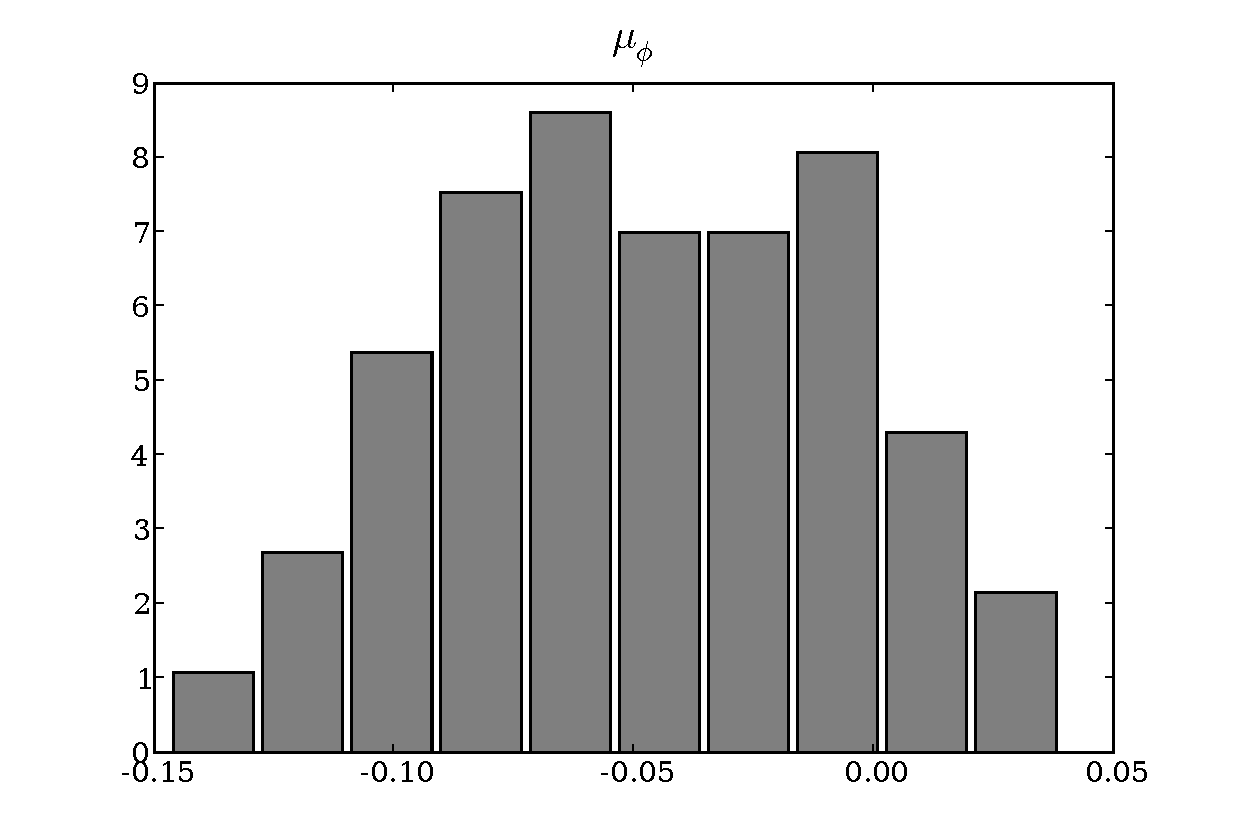
\epsfig{file=figs/ESSmuphiPosterior.pdf,width=7cm}
% %         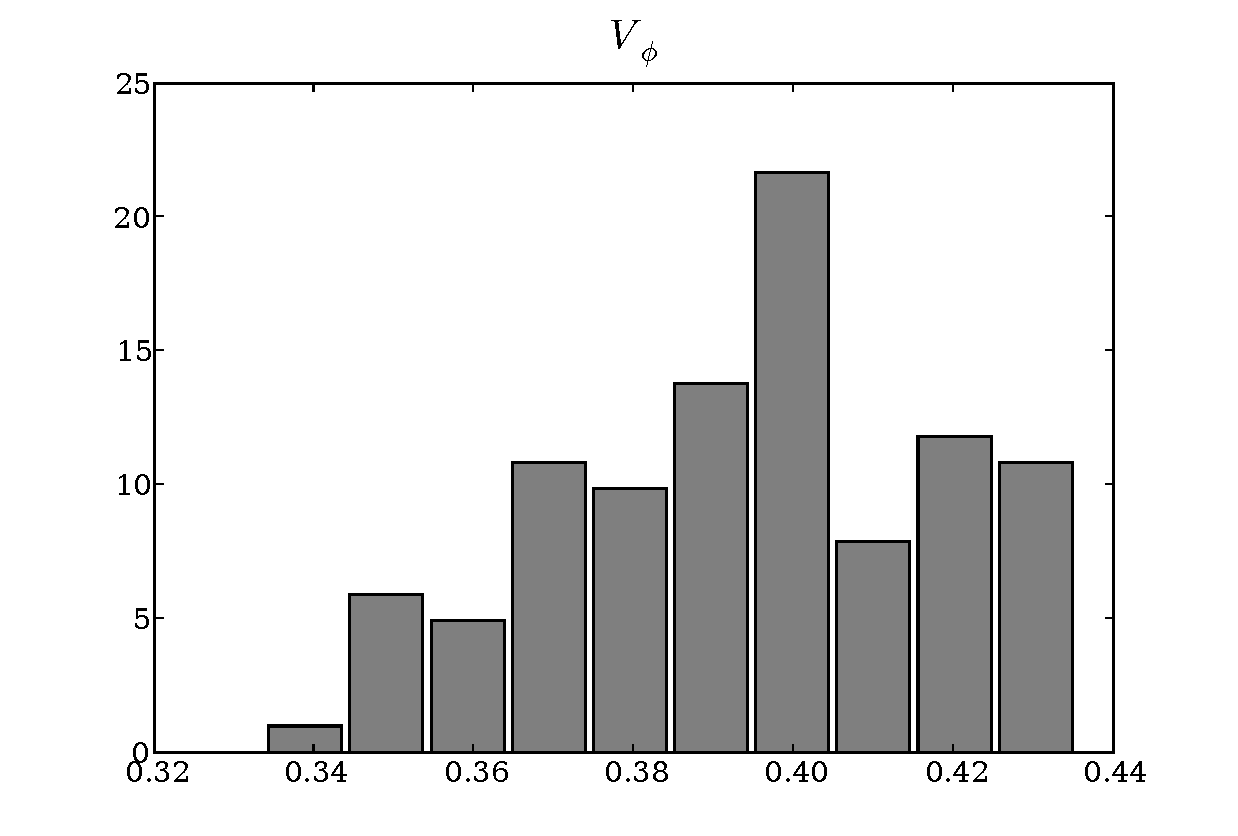
\epsfig{file=figs/ESSVphiPosterior.pdf,width=7cm}
% %         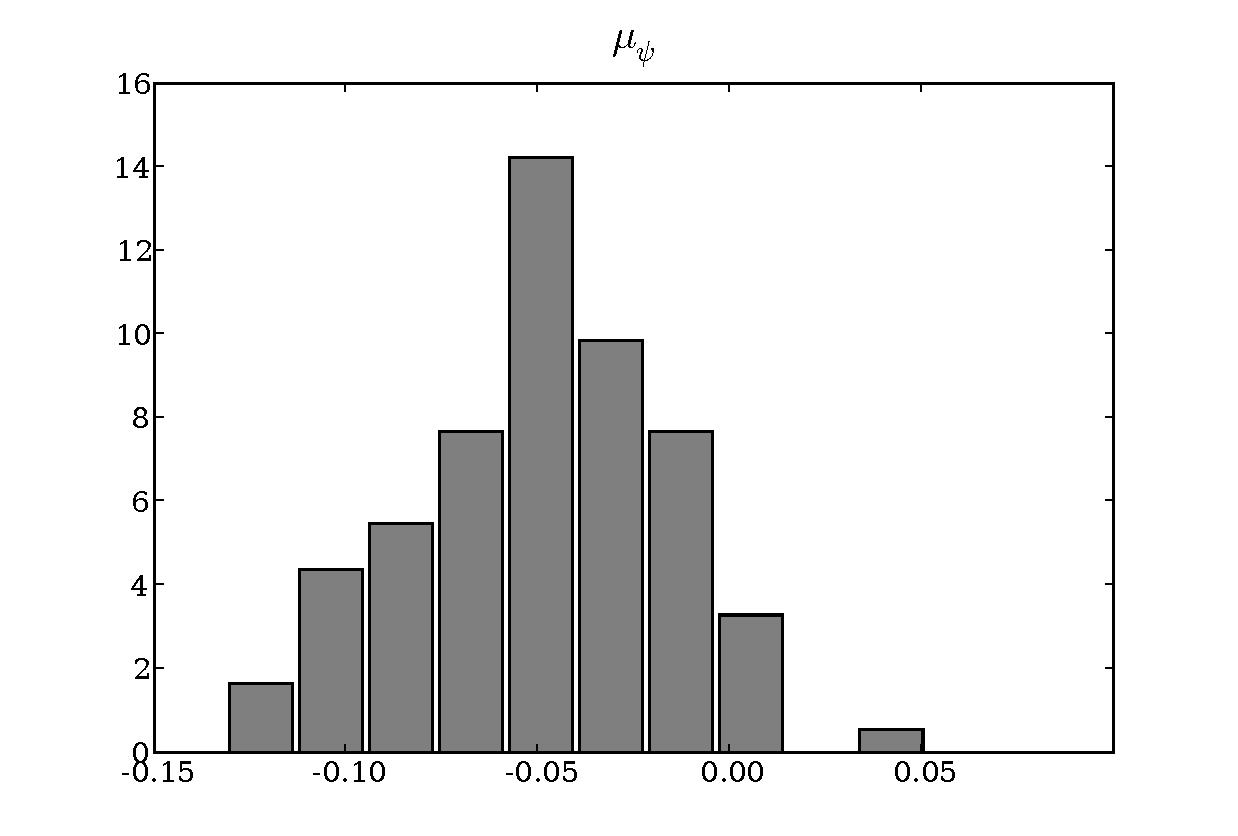
\epsfig{file=figs/ESSmupsiPosterior.pdf,width=7cm}
% %         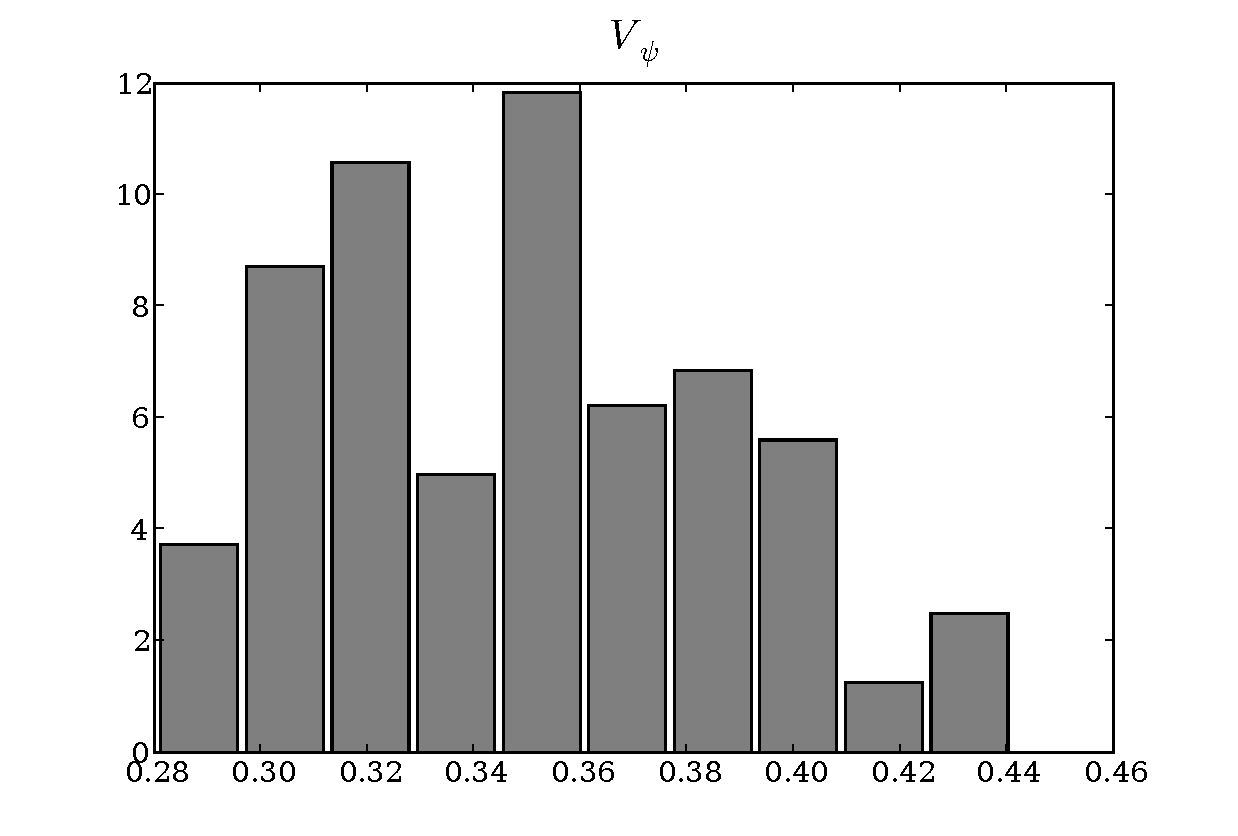
\epsfig{file=figs/ESSVpsiPosterior.pdf,width=7cm}
% %     \caption{caption}
% %     \label{fig:ESSphipsi}
% % \end{figure}
% %
% % \begin{figure}
% %     \centering
% %         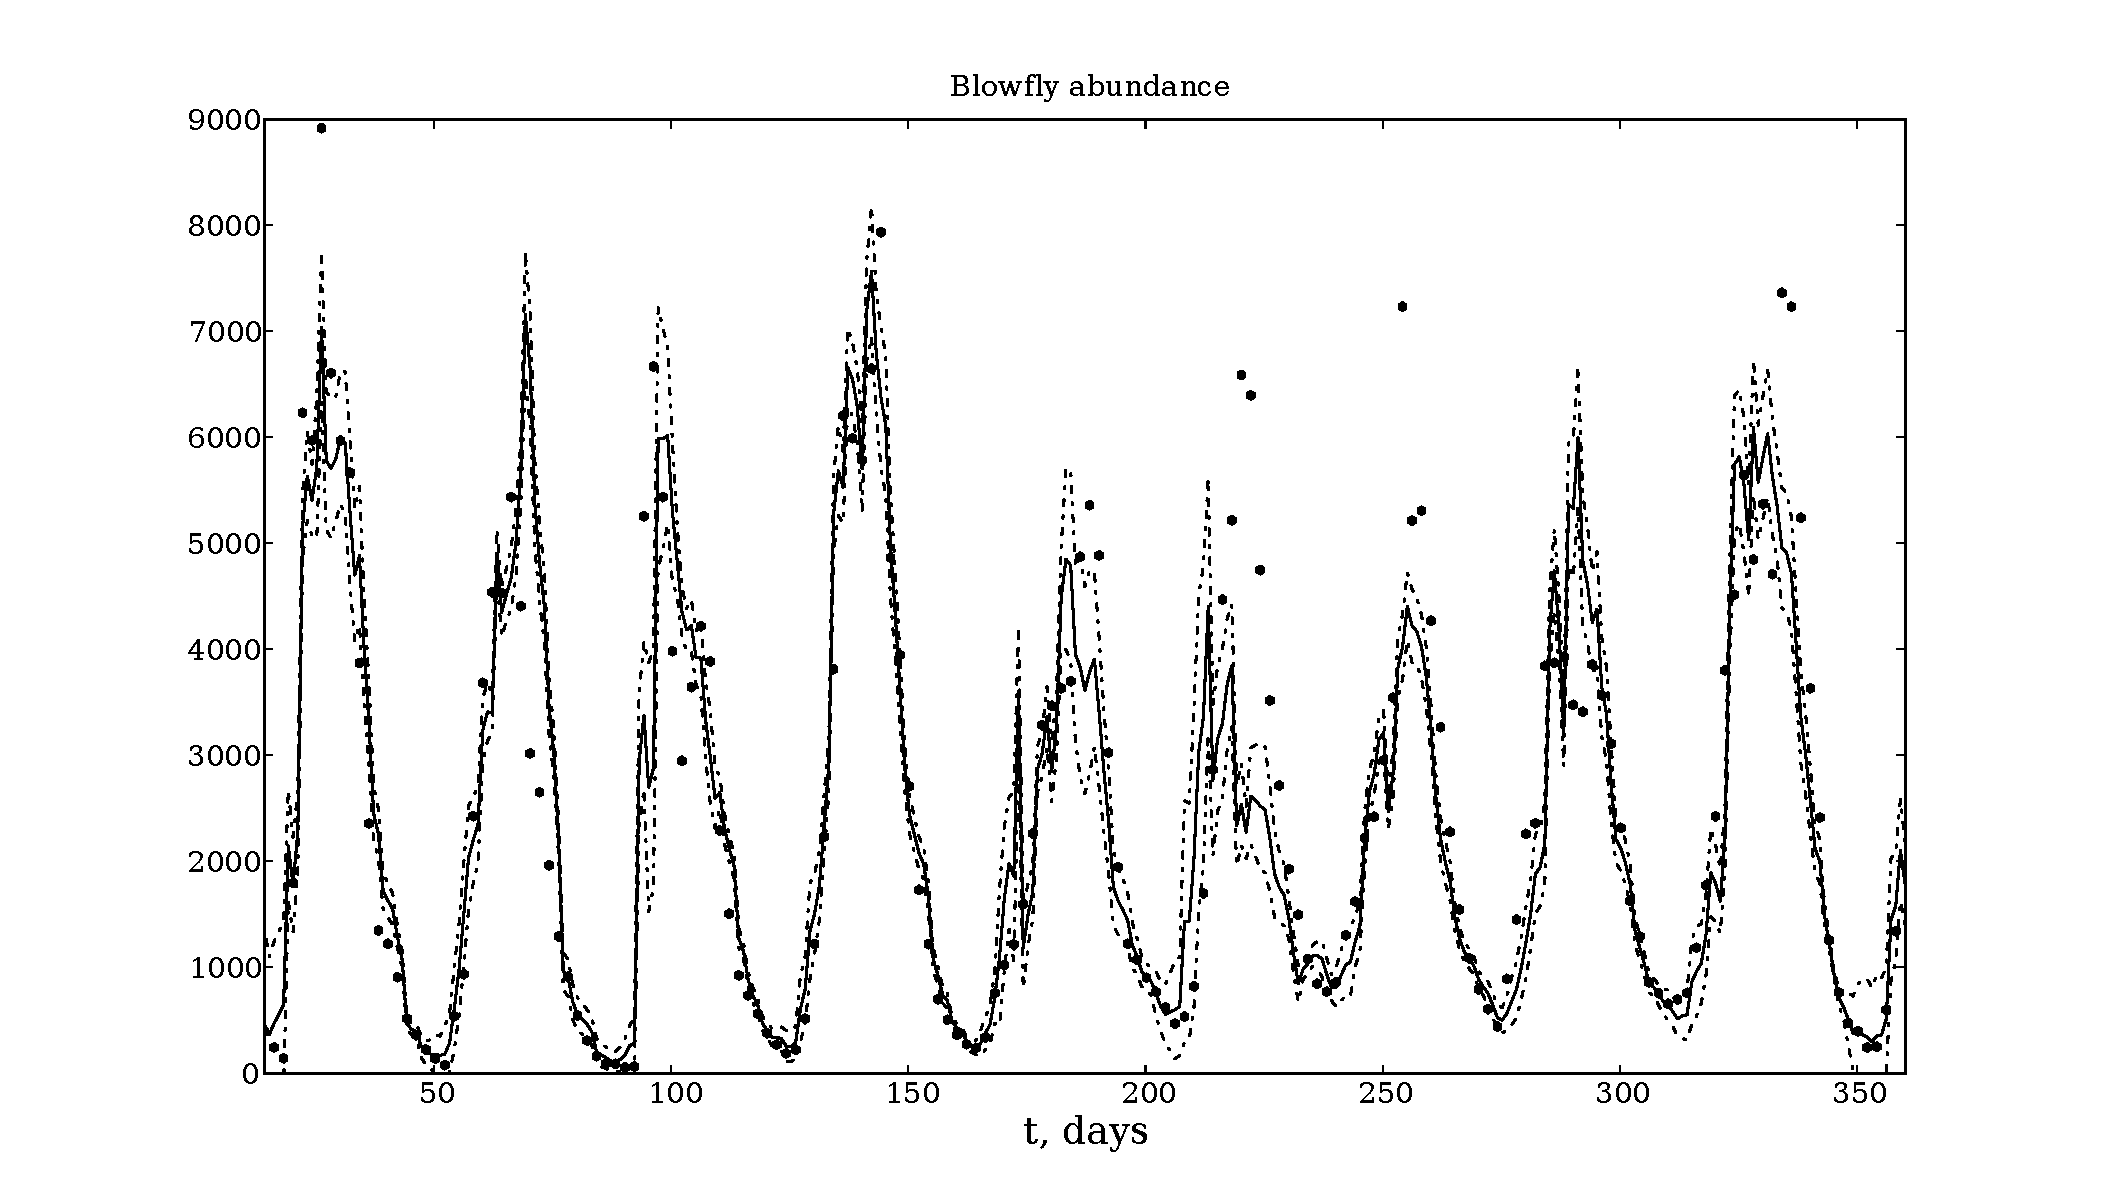
\epsfig{file=figs/ESSblowflyfit.pdf,width=15cm}
% %     \caption{caption}
% %     \label{fig:ESSfit}
% % \end{figure}
%
